% !TEX program = xelatex
\documentclass[11pt,oneside]{book}

% ==============================================================================
% 1. CÁC THƯ VIỆN & CẤU HÌNH GÓI (PACKAGES)
% ==============================================================================
\usepackage{silence}
\WarningFilter{tcolorbox}{Using nobreak failed}
\WarningFilter{babel}{No hyphenation patterns}
\WarningFilter{microtype}{Unable to apply patch}
\WarningFilter{rerunfilecheck}{File `main.out'}
\WarningFilter{latex}{Overfull}
\WarningFilter{latex}{Underfull}

\usepackage{fontspec}
\usepackage[vietnamese]{babel}
\shorthandoff{"}

\usepackage[
    paper=a4paper,
    top=2.6cm,
    bottom=2.6cm,
    left=2.5cm,
    right=2.5cm,
    headheight=26pt,
    headsep=20pt,
    footskip=30pt
]{geometry}

\usepackage{xcolor}
\usepackage{colortbl}
\definecolor{primaryBlue}{HTML}{0F4C81}     % Classic Navy/Royal Blue
\definecolor{secondaryTeal}{HTML}{008080}   % Teal Accent
\definecolor{darkText}{HTML}{1A1A1A}        % Màu chữ đen dịu
\definecolor{accentOrange}{HTML}{E65100}    % Cam điểm nhấn
\definecolor{accentPurple}{HTML}{5E35B1}    % Tím sang trọng
\definecolor{codeBg}{HTML}{F8FAFC}          % Nền code Slate nhạt
\definecolor{slateBg}{HTML}{F1F5F9}         % Nền UI Slate trung tính
\definecolor{codeBorder}{HTML}{CBD5E1}      % Viền code Slate
\definecolor{codeComment}{HTML}{64748B}     % Màu chú thích Slate
\definecolor{codeKeyword}{HTML}{D97706}     % Từ khóa Cam/Hổ phách đậm
\definecolor{codeString}{HTML}{059669}      % Chuỗi ký tự Emerald
\definecolor{codeKey}{HTML}{0284C7}         % Tên thuộc tính Cyan
\definecolor{codeNumber}{HTML}{7C3AED}      % Giá trị số Indigo

\definecolor{noteBg}{HTML}{F0F7FF}
\definecolor{noteBorder}{HTML}{0F4C81}
\definecolor{tipBg}{HTML}{F0FDF4}
\definecolor{tipBorder}{HTML}{16A34A}
\definecolor{warnBg}{HTML}{FFFBEB}
\definecolor{warnBorder}{HTML}{D97706}
\definecolor{conceptBg}{HTML}{F5F3FF}
\definecolor{conceptBorder}{HTML}{7C3AED}
\definecolor{successGreen}{HTML}{16A34A}
\definecolor{dangerRed}{HTML}{DC2626}

\usepackage{graphicx}
\usepackage{float}
\usepackage{caption}
\usepackage{subcaption}
\usepackage{tikz}
\usetikzlibrary{shapes, shadows, arrows.meta, positioning, calc, decorations.pathreplacing, fit}

\usepackage{tabularx}
\usepackage{booktabs}
\usepackage{multirow}
\usepackage{array}
\usepackage{ragged2e}

\usepackage[most]{tcolorbox}
\usepackage{listings}
\usepackage{fancyhdr}
\usepackage{titlesec}
\usepackage{titletoc}

\usepackage{hyperref}
\hypersetup{
    colorlinks=true,
    linkcolor=primaryBlue,
    citecolor=secondaryTeal,
    urlcolor=accentOrange,
    pdfauthor={Đội Ngũ Lập Trình Web},
    pdftitle={Giáo Trình CSS3 - Tập 2: Bố Cục Hiện Đại, Box Model \& Kỹ Thuật Chuyên Sâu},
    pdfkeywords={CSS3, Box Model, Flexbox, Grid, Responsive Design, CSS Variables, BEM, Animations, XeLaTeX}
}

\usepackage{indentfirst}
\setlength{\parindent}{18pt}
\setlength{\parskip}{2pt}

\usepackage{enumitem}
\usepackage[normalem]{ulem}
\setlist[itemize]{leftmargin=1.8em, itemsep=2pt, parsep=0pt, topsep=3pt, partopsep=0pt}
\setlist[enumerate]{leftmargin=1.8em, itemsep=2pt, parsep=0pt, topsep=3pt, partopsep=0pt}

\usepackage{setspace}
\setstretch{1.15}
\usepackage{needspace}
\usepackage{seqsplit}

% ==============================================================================
% 2. ĐỊNH NGHĨA KHUNG HỘP (CALLOUT BOXES) & NÂNG CAO (COMMANDS)
% ==============================================================================
\hfuzz=500pt
\vfuzz=500pt
\hbadness=10000
\vbadness=10000
\tcbset{lines before break=1}

\newtcolorbox{noteBox}[1][Ghi Chú Quan Trọng]{
    enhanced,
    before=\par\vspace{6pt}\noindent,
    after=\par\vspace{6pt},
    width=\linewidth,
    colback=noteBg,
    colframe=noteBorder,
    boxrule=0.5pt,
    arc=5pt,
    title={\small\sffamily\bfseries\color{noteBorder} [Ghi Chú]\quad #1},
    coltitle=noteBorder,
    fonttitle=\bfseries\sffamily,
    fontupper=\RaggedRight,
    attach title to upper,
    after title={\par\vspace{3pt}{\color{noteBorder!20}\hrule height 0.5pt}\par\vspace{5pt}},
    top=7pt, bottom=7pt, left=12pt, right=12pt
}

\newtcolorbox{tipBox}[1][Mẹo Thực Hành]{
    enhanced,
    before=\par\vspace{6pt}\noindent,
    after=\par\vspace{6pt},
    width=\linewidth,
    colback=tipBg,
    colframe=tipBorder,
    boxrule=0.5pt,
    arc=5pt,
    title={\small\sffamily\bfseries\color{tipBorder} [Mẹo]\quad #1},
    coltitle=tipBorder,
    fonttitle=\bfseries\sffamily,
    fontupper=\RaggedRight,
    attach title to upper,
    after title={\par\vspace{3pt}{\color{tipBorder!20}\hrule height 0.5pt}\par\vspace{5pt}},
    top=7pt, bottom=7pt, left=12pt, right=12pt
}

\newtcolorbox{warnBox}[1][Cảnh Báo \& Lỗi Thường Gặp]{
    enhanced,
    before=\par\vspace{6pt}\noindent,
    after=\par\vspace{6pt},
    width=\linewidth,
    colback=warnBg,
    colframe=warnBorder,
    boxrule=0.5pt,
    arc=5pt,
    title={\small\sffamily\bfseries\color{warnBorder} [Cảnh Báo]\quad #1},
    coltitle=warnBorder,
    fonttitle=\bfseries\sffamily,
    fontupper=\RaggedRight,
    attach title to upper,
    after title={\par\vspace{3pt}{\color{warnBorder!20}\hrule height 0.5pt}\par\vspace{5pt}},
    top=7pt, bottom=7pt, left=12pt, right=12pt
}

\newtcolorbox{conceptBox}[1][Khái Niệm Cốt Lõi]{
    enhanced,
    before=\par\vspace{6pt}\noindent,
    after=\par\vspace{6pt},
    width=\linewidth,
    colback=conceptBg,
    colframe=conceptBorder,
    boxrule=0.5pt,
    arc=5pt,
    title={\small\sffamily\bfseries\color{conceptBorder} [Khái Niệm]\quad #1},
    coltitle=conceptBorder,
    fonttitle=\bfseries\sffamily,
    fontupper=\RaggedRight,
    attach title to upper,
    after title={\par\vspace{3pt}{\color{conceptBorder!20}\hrule height 0.5pt}\par\vspace{5pt}},
    top=7pt, bottom=7pt, left=12pt, right=12pt
}

\newcommand{\macDots}{%
  \tikz[baseline=-0.5ex]{
    \fill[color=red!75!black] (0,0) circle (3pt);
    \fill[color=yellow!85!black] (8pt,0) circle (3pt);
    \fill[color=green!75!black] (16pt,0) circle (3pt);
  }\hspace{8pt}%
}

\newtcolorbox{codeWindow}[1][Cửa Sổ Mã Nguồn]{
    enhanced,
    before=\par\vspace{8pt}\noindent,
    after=\par\vspace{8pt},
    width=\linewidth,
    colback=codeBg,
    colframe=primaryBlue!30,
    colbacktitle=primaryBlue!8,
    boxrule=0.8pt,
    arc=7pt,
    title={\macDots \small\sffamily\bfseries\color{primaryBlue} #1},
    coltitle=primaryBlue,
    fonttitle=\bfseries\sffamily,
    top=6pt, bottom=4pt, left=8pt, right=8pt,
    toptitle=5pt, bottomtitle=5pt, lefttitle=10pt, righttitle=10pt
}

\newtcolorbox{codeWindowBreakable}[1][Cửa Sổ Mã Nguồn]{
    enhanced,
    breakable,
    before=\par\vspace{8pt}\noindent,
    after=\par\vspace{8pt},
    width=\linewidth,
    colback=codeBg,
    colframe=primaryBlue!30,
    colbacktitle=primaryBlue!8,
    boxrule=0.8pt,
    arc=7pt,
    title={\macDots \small\sffamily\bfseries\color{primaryBlue} #1},
    coltitle=primaryBlue,
    fonttitle=\bfseries\sffamily,
    top=6pt, bottom=2pt, left=8pt, right=8pt,
    toptitle=5pt, bottomtitle=5pt, lefttitle=10pt, righttitle=10pt
}

\newtcolorbox{browserWindow}[1][Mô Phỏng Trình Duyệt Web]{
    enhanced,
    before=\par\vspace{10pt}\noindent,
    after=\par\vspace{10pt},
    width=\linewidth,
    colback=white,
    colframe=primaryBlue!35,
    colbacktitle=gray!10,
    boxrule=0.8pt,
    arc=8pt,
    title={%
        \macDots \;\; {\small\sffamily\bfseries\color{primaryBlue} BROWSER PREVIEW} \hfill
        {\normalfont\small\sffamily\bfseries\color{darkText} #1}%
    },
    coltitle=darkText,
    fonttitle=\bfseries\sffamily,
    top=10pt, bottom=10pt, left=14pt, right=14pt,
    toptitle=6pt, bottomtitle=6pt, lefttitle=10pt, righttitle=10pt
}

\newtcolorbox{prettyTableBox}[1][Bảng Thống Kê]{
    enhanced,
    before=\par\vspace{8pt}\needspace{4.5\baselineskip}\noindent,
    after=\par\vspace{8pt},
    width=\linewidth,
    colback=white,
    colframe=primaryBlue!30,
    colbacktitle=primaryBlue!8,
    boxrule=0.8pt,
    arc=7pt,
    title={\small\sffamily\bfseries\color{primaryBlue} [Bảng]\quad #1},
    coltitle=primaryBlue,
    fonttitle=\bfseries\sffamily,
    top=0pt, bottom=0pt, left=0pt, right=0pt,
    toptitle=5pt, bottomtitle=5pt, lefttitle=10pt, righttitle=10pt
}

\renewcommand{\arraystretch}{1.2}
\arrayrulecolor{primaryBlue!20}

\newcolumntype{C}[1]{>{\centering\arraybackslash}m{#1}}
\newcolumntype{L}[1]{>{\raggedright\arraybackslash}m{#1}}
\newcolumntype{Y}{>{\centering\arraybackslash}X}
\newcolumntype{Z}{>{\raggedright\arraybackslash}X}
\newcolumntype{K}[1]{>{\ttfamily\color{accentOrange}\bfseries\raggedright\arraybackslash}m{#1}}

\newcommand{\thd}[1]{\textcolor{white}{\textbf{\strut #1}}}
\newcommand{\codeinline}[1]{\textcolor{accentOrange}{\texttt{#1}}}
\newcommand{\term}[1]{\textbf{\textcolor{primaryBlue}{#1}}}
\newcommand{\badge}[1]{\tcbox[on line, arc=3pt, colback=primaryBlue!10, colframe=primaryBlue!30, boxsep=1pt, left=3pt, right=3pt, top=1pt, bottom=1pt]{\small\sffamily\color{primaryBlue}#1}}
\DeclareRobustCommand{\taghint}[1]{\texorpdfstring{\textcolor{accentOrange}{\textbf{\texttt{#1}}}}{#1}}
\DeclareRobustCommand{\csshint}[1]{\texorpdfstring{\textcolor{accentOrange}{\textbf{\texttt{#1}}}}{#1}}

% ==============================================================================
% 3. CẤU HÌNH MÃ NGUỒN (CODE LISTINGS & UNICODE)
% ==============================================================================
\lstdefinelanguage{JavaScript}{
    keywords={break, case, catch, class, const, continue, debugger, default, delete, do, else, export, extends, false, finally, for, function, if, import, in, instanceof, new, null, return, super, switch, this, throw, true, try, typeof, var, void, while, with, yield, async, await, let},
    keywordstyle=\color{codeKeyword}\bfseries,
    ndkeywords={class, export, default, boolean, throw, implements, import, this, fetch, console, log, then},
    ndkeywordstyle=\color{codeKey}\bfseries,
    identifierstyle=\color{darkText},
    sensitive=true,
    comment=[l]{//},
    morecomment=[s]{/*}{*/},
    commentstyle=\color{codeComment}\upshape,
    stringstyle=\color{codeString},
    morestring=[b]',
    morestring=[b]",
    morestring=[b]`
}

\lstdefinelanguage{HTML5}{
    language=html,
    sensitive=true,
    alsoletter={<>=-/},
    morekeywords={
        <!DOCTYPE, html, head, title, meta, link, script, body,
        header, nav, main, section, article, aside, footer,
        h1, h2, h3, h4, h5, h6, p, a, img, ul, ol, li, div, span,
        form, input, button, select, option, textarea, label, table, tr, td, th,
        figure, figcaption, details, summary, dialog, meter, progress, picture, source, video, audio, track, iframe, svg, canvas, math
    },
    keywordstyle=\color{primaryBlue}\bfseries,
    tag=[s]{<}{>},
    tagstyle=\color{primaryBlue}\bfseries,
    stringstyle=\color{codeString},
    morestring=[b]",
    comment=[s]{<!--}{-->},
    commentstyle=\color{codeComment}\upshape
}

\lstdefinelanguage{CSS3}{
    keywords={color, background, background-color, border, border-radius, padding, margin, margin-bottom, font-weight, font-size, display, flex, grid, width, height, appearance, box-sizing, outline, outline-offset, box-shadow},
    keywordstyle=\color{primaryBlue}\bfseries,
    sensitive=false,
    comment=[s]{/*}{*/},
    commentstyle=\color{codeComment}\upshape,
    stringstyle=\color{codeString},
    morestring=[b]",
    morestring=[b]'
}
\lstdefinelanguage{CSS}{language=CSS3}

\lstdefinestyle{webcode}{
    backgroundcolor=\color{codeBg},
    basicstyle=\ttfamily\small,
    columns=fullflexible,
    keepspaces=true,
    breakatwhitespace=false,
    breaklines=true,
    captionpos=b,
    deletekeywords={...},
    escapeinside={(*@}{@*)},
    extendedchars=false,
    inputencoding=utf8,
    firstnumber=1,
    frame=none,
    rulecolor=\color{codeBorder},
    language=CSS3,
    numbersep=8pt,
    numbers=left,
    numberstyle=\ttfamily\scriptsize\color{codeComment},
    showspaces=false,
    showstringspaces=false,
    showtabs=false,
    stepnumber=1,
    tabsize=2,
    aboveskip=3pt,
    belowskip=1pt,
    xleftmargin=16pt,
    xrightmargin=4pt
}

\lstset{style=webcode}

% ==============================================================================
% 4. PHÔNG CHỮ & ĐỊNH DẠNG TIÊU ĐỀ (TITLES & FONTS)
% ==============================================================================
\setmainfont{Times New Roman}[
    BoldFont = Times New Roman Bold,
    ItalicFont = Times New Roman Italic,
    BoldItalicFont = Times New Roman Bold Italic
]
\setsansfont{Arial}[
    BoldFont = Arial Bold,
    ItalicFont = Arial Italic,
    BoldItalicFont = Arial Bold Italic
]
\setmonofont{Consolas}[Scale=0.92]

\titleformat{\chapter}[display]
  {\normalfont\sffamily}
  {
    \begin{tikzpicture}
      \node[fill=primaryBlue, text=white, font=\sffamily\bfseries\small, inner xsep=10pt, inner ysep=4pt, rounded corners=3pt] {CHƯƠNG \thechapter};
    \end{tikzpicture}
  }
  {6pt}
  {\Huge\bfseries\color{darkText}\raggedright}
  [\vspace{8pt}{\color{primaryBlue}\hrule height 1.5pt}\vspace{15pt}]

\titlespacing*{\chapter}{0pt}{-10pt}{20pt}

\titleformat{name=\chapter,numberless}[block]
  {\normalfont\huge\sffamily\bfseries\color{primaryBlue}}
  {}
  {0pt}
  {}

\titlespacing*{name=\chapter,numberless}{0pt}{10pt}{20pt}

\titleformat{\section}
  {\normalfont\Large\sffamily\bfseries\color{primaryBlue}}
  {\textcolor{primaryBlue}{\rule[-0.2ex]{3.5pt}{1.15em}}\hspace{8pt}\thesection}
  {8pt}
  {}

\titleformat{name=\section,numberless}
  {\normalfont\Large\sffamily\bfseries\color{primaryBlue}}
  {\textcolor{primaryBlue}{\rule[-0.2ex]{3.5pt}{1.15em}}}
  {8pt}
  {}

\titlespacing*{\section}{0pt}{14pt}{7pt}
\titlespacing*{name=\section,numberless}{0pt}{14pt}{7pt}

\titleformat{\subsection}
  {\normalfont\large\sffamily\bfseries\color{secondaryTeal}}
  {\textcolor{secondaryTeal}{\rule[-0.15ex]{2.5pt}{1.05em}}\hspace{7pt}\thesubsection}
  {7pt}
  {}

\titleformat{name=\subsection,numberless}
  {\normalfont\large\sffamily\bfseries\color{secondaryTeal}}
  {\textcolor{secondaryTeal}{\rule[-0.15ex]{2.5pt}{1.05em}}}
  {7pt}
  {}

\titlespacing*{\subsection}{0pt}{10pt}{5pt}
\titlespacing*{name=\subsection,numberless}{0pt}{10pt}{5pt}

% ==============================================================================
% 5. CẤU HÌNH HEADER & FOOTER
% ==============================================================================
\pagestyle{fancy}
\fancyhf{}
\fancyhead[R]{\sffamily\small\color{darkText}\rightmark}
\fancyfoot[R]{\sffamily\bfseries\color{primaryBlue}\thepage}
\fancyfoot[C]{\sffamily\small\color{codeComment}Giáo Trình CSS3 -- Tập 2: Bố Cục Hiện Đại \& Kỹ Thuật Chuyên Sâu}

\renewcommand{\headrulewidth}{0.6pt}
\renewcommand{\headrule}{{\color{primaryBlue!40}\hrule width\headwidth height\headrulewidth}}
\renewcommand{\footrulewidth}{0.4pt}
\renewcommand{\footrule}{{\color{codeBorder}\hrule width\headwidth height\footrulewidth}}

\fancypagestyle{plain}{
  \fancyhf{}
  \fancyfoot[R]{\sffamily\bfseries\color{primaryBlue}\thepage}
  \renewcommand{\headrulewidth}{0pt}
  \renewcommand{\footrulewidth}{0.4pt}
}

% ==============================================================================
% BẮT ĐẦU TÀI LIỆU
% ==============================================================================
\begin{document}
\shorthandoff{"}

% ------------------------------------------------------------------------------
% TRANG BÌA CHÍNH (MAIN COVER PAGE - CSS3 TẬP 2)
% ------------------------------------------------------------------------------
\begin{titlepage}
    \begin{tikzpicture}[remember picture, overlay]
        % Khối Nền Xanh Navy Sang Trọng Đỉnh Trang (Top Banner)
        \fill[primaryBlue] (current page.north west) -- (current page.north east) -- ($(current page.north east)+(0,-10.5cm)$) -- ($(current page.north west)+(0,-8.5cm)$) -- cycle;
        
        % Dải Cam Điểm Nhấn Sắc Nét (Accent Orange Strip)
        \fill[accentOrange] ($(current page.north west)+(0,-8.5cm)$) -- ($(current page.north east)+(0,-10.5cm)$) -- ($(current page.north east)+(0,-10.9cm)$) -- ($(current page.north west)+(0,-8.9cm)$) -- cycle;
        
        % Mảng Họa Tiết Trang Trí Hiện Đại Ở Góc Phải
        \fill[white!12] ($(current page.north east)+(-6.5cm,0)$) -- (current page.north east) -- ($(current page.north east)+(0,-5.0cm)$) -- cycle;
        \fill[secondaryTeal!25] ($(current page.north east)+(-3.2cm,0)$) -- (current page.north east) -- ($(current page.north east)+(0,-2.5cm)$) -- cycle;

        % Thanh Nền Chân Trang (Bottom Accent Bar)
        \fill[primaryBlue] ($(current page.south west)+(0,0)$) rectangle ($(current page.south east)+(0,1.3cm)$);
        \fill[accentOrange] ($(current page.south west)+(0,1.3cm)$) rectangle ($(current page.south east)+(0,1.48cm)$);

        % --- NỘI DUNG NỔI BẬT TRÊN BÌA ---
        
        % 1. Header Đơn Vị Phát Hành & Nhãn Tập 2
        \node[anchor=north west] at ($(current page.north west)+(2.2cm,-1.5cm)$) {
            {\sffamily \bfseries \small \color{white!85} GIÁO TRÌNH ĐÀO TẠO KỸ SƯ FRONTEND CHUYÊN SÂU}
        };

        % 2. Tiêu Đề Chính & Phụ
        \node[anchor=north west, text width=16cm] at ($(current page.north west)+(2.2cm,-2.7cm)$) {
            {\fontsize{34pt}{40pt}\selectfont \sffamily \bfseries \color{white} GIÁO TRÌNH CSS3} \\[0.35cm]
            {\fontsize{24pt}{30pt}\selectfont \sffamily \bfseries \color{accentOrange} TẬP 2: BỐ CỤC HIỆN ĐẠI \& NÂNG CAO} \\[0.5cm]
            {\large \sffamily \color{white!95} Chuyên Đề Box Model, Outline, Flexbox, CSS Grid, Responsive \& Animations}
        };

        % 3. Badge Capsule Nhóm Công Nghệ Nổi Bật
        \node[anchor=north] at ($(current page.north)+(0,-8.7cm)$) {
            \begin{tcolorbox}[
                on line,
                colback=white,
                colframe=primaryBlue!40,
                boxrule=1.2pt,
                arc=16pt,
                left=18pt, right=18pt, top=8pt, bottom=8pt,
                drop shadow=black!12!white
            ]
                {\sffamily \bfseries \small \color{primaryBlue}
                \textcolor{accentOrange}{\rule{4.5pt}{4.5pt}}\; CSS Box Model \quad$\bullet$\quad 
                \textcolor{accentOrange}{\rule{4.5pt}{4.5pt}}\; Flexbox \& Grid \quad$\bullet$\quad 
                \textcolor{accentOrange}{\rule{4.5pt}{4.5pt}}\; Responsive Web \quad$\bullet$\quad 
                \textcolor{accentOrange}{\rule{4.5pt}{4.5pt}}\; Animations}
            \end{tcolorbox}
        };

        % 4. Khối Giới Thiệu Trọng Tâm (Card Trung Tâm)
        \node[anchor=center, text width=15.5cm, align=center] at ($(current page.center)+(0,-2.3cm)$) {
            \begin{tcolorbox}[
                colback=white,
                colframe=primaryBlue!25,
                boxrule=1pt,
                arc=10pt,
                top=16pt, bottom=16pt, left=20pt, right=20pt,
                drop shadow=black!6!white
            ]
                \centering
                {\Large \sffamily \bfseries \color{primaryBlue} TÀI LIỆU CHUYÊN SÂU TẬP TRUNG CSS3 -- TẬP 2} \\[0.3cm]
                {\color{accentOrange}\rule{6cm}{1.2pt}} \\[0.35cm]
                {\normalsize \sffamily \bfseries \color{darkText} 
                Làm Chủ Mô Hình Hộp (Box Model) $\bullet$ Bố Cục Một Chiều Flexbox \& Hai Chiều CSS Grid} \\[0.25cm]
                {\small \sffamily \color{codeComment} 
                Hệ thống hóa toàn diện phương pháp dàn trang hiện đại $\bullet$ Thiết kế Responsive thích ứng đa màn hình $\bullet$ Tối ưu hiệu năng render chuẩn kỹ sư UI/UX}
            \end{tcolorbox}
        };

        % 5. Thông tin Xuất Bản Chân Trang
        \node[anchor=south west, align=left] at ($(current page.south west)+(2.2cm,1.9cm)$) {
            {\sffamily \bfseries \small \color{primaryBlue} ĐỘI NGŨ BIÊN SOẠN WEB} \\
            {\sffamily \scriptsize \color{codeComment} Tài liệu lưu hành nội bộ}
        };

        \node[anchor=south east, align=right] at ($(current page.south east)+(-2.2cm,1.9cm)$) {
            {\sffamily \bfseries \small \color{primaryBlue} NĂM 2026} \\
            {\sffamily \scriptsize \color{codeComment} Phiên bản Standalone Tập 2}
        };

        \node[anchor=south, color=white, font=\sffamily\scriptsize\bfseries] at ($(current page.south)+(0,0.5cm)$) {
            CHINH PHỤC BỐ CỤC HIỆN ĐẠI \& NGHỆ THUẬT DÀN TRANG CSS3 CHUYÊN NGHIỆP
        };
    \end{tikzpicture}
\end{titlepage}

% ------------------------------------------------------------------------------
% TRANG BÌA PHỤ (SECONDARY COVER PAGE)
% ------------------------------------------------------------------------------
\clearpage
\thispagestyle{empty}
\begin{tikzpicture}[remember picture, overlay]
    % Khung Viền Kép Sang Trọng (Double Border)
    \draw[primaryBlue, line width=1.4pt] 
        ($(current page.north west)+(2.0cm,-2.0cm)$) rectangle ($(current page.south east)+(-2.0cm,2.0cm)$);
    \draw[accentOrange, line width=0.7pt] 
        ($(current page.north west)+(2.15cm,-2.15cm)$) rectangle ($(current page.south east)+(-2.15cm,2.15cm)$);

    \node[anchor=north, align=center, text width=15cm] at ($(current page.north)+(0,-3.5cm)$) {
        {\small \sffamily \bfseries \color{primaryBlue} ĐỘI NGŨ BIÊN SOẠN WEB} \\[0.2cm]
        {\scriptsize \sffamily \color{codeComment} TÀI LIỆU LƯU HÀNH NỘI BỘ -- CHUYÊN ĐỀ CSS3 TẬP 2}
    };

    \node[anchor=center, align=center, text width=15cm] at ($(current page.center)+(0,2.2cm)$) {
        {\fontsize{28pt}{34pt}\selectfont \sffamily \bfseries \color{primaryBlue} GIÁO TRÌNH CSS3} \\[0.4cm]
        {\fontsize{20pt}{26pt}\selectfont \sffamily \bfseries \color{accentOrange} TẬP 2: BỐ CỤC HIỆN ĐẠI \& NÂNG CAO} \\[0.6cm]
        {\large \sffamily \color{darkText} Box Model, Outline, Flexbox, Grid, Responsive \& Animations}
    };

    \draw[primaryBlue!35, line width=0.8pt] ($(current page.center)+(-4cm,-0.8cm)$) -- ($(current page.center)+(4cm,-0.8cm)$);

    \node[anchor=center, align=center, text width=15cm] at ($(current page.center)+(0,-2.6cm)$) {
        {\large \sffamily \bfseries \color{primaryBlue} TẬP TRUNG BIÊN SOẠN \& THỰC HÀNH CSS3 NÂNG CAO} \\[0.3cm]
        {\small \sffamily \color{codeComment} Biên soạn chi tiết $\bullet$ Minh họa trực quan $\bullet$ Sẵn sàng tích hợp nội dung mới}
    };

    \node[anchor=south, align=center, text width=15cm] at ($(current page.south)+(0,3.2cm)$) {
        {\sffamily \bfseries \small \color{primaryBlue} NĂM 2026} \\[0.1cm]
        {\sffamily \scriptsize \color{darkText} Phiên bản Standalone Tập 2 -- XeLaTeX Unicode}
    };
\end{tikzpicture}
\clearpage

% ==============================================================================
% MỤC LỤC TÀI LIỆU (TABLE OF CONTENTS)
% ==============================================================================
\frontmatter
\renewcommand{\contentsname}{MỤC LỤC}
\setcounter{tocdepth}{2}

\makeatletter
\renewcommand{\tableofcontents}{%
  \chapter*{\contentsname}%
  {\color{accentOrange}\rule{3.5cm}{2.5pt}}\\[3pt]%
  {\sffamily\small\color{codeComment}\itshape
   Giáo Trình Chuyên Sâu CSS3 \textendash{} Tập 2: Bố Cục Hiện Đại \& Kỹ Thuật Chuyên Sâu}%
  \par\vspace{16pt}%
  \@starttoc{toc}%
}
\makeatother

\contentsmargin{2.2em}

\titlecontents{part}[0pt]
  {\addvspace{20pt}\sffamily\large\bfseries\color{primaryBlue}}
  {}
  {}
  {\hfill\textbf{\color{primaryBlue}\contentspage}}
  [\addvspace{5pt}{\color{primaryBlue!25}\hrule height 0.8pt}\addvspace{6pt}]

\titlecontents{chapter}[0pt]
  {\addvspace{12pt}\sffamily\normalsize\bfseries\color{darkText}}
  {\textcolor{primaryBlue}{Chương\ \thecontentslabel:\enskip}}
  {\textcolor{primaryBlue}{}}
  {\enspace\titlerule*[0.5pc]{\textcolor{primaryBlue!30}{.}}\enspace\textbf{\color{primaryBlue}\contentspage}}
  [\addvspace{3pt}]

\titlecontents{section}[1.8em]
  {\addvspace{4pt}\sffamily\normalsize\color{darkText}}
  {\textcolor{primaryBlue}{\bfseries\thecontentslabel}\enskip}
  {\textcolor{darkText}{}}
  {\enspace\titlerule*[0.5pc]{\textcolor{gray!35}{.}}\enspace\textcolor{darkText}{\contentspage}}
  [\addvspace{1pt}]

\titlecontents{subsection}[3.8em]
  {\addvspace{1.5pt}\sffamily\small\color{darkText!75}}
  {\textcolor{secondaryTeal!80}{\thecontentslabel}\enskip}
  {\textcolor{darkText!75}{}}
  {\enspace\titlerule*[0.5pc]{\textcolor{gray!22}{.}}\enspace\textcolor{darkText!70}{\contentspage}}
  []

\begingroup
\setlength{\parskip}{0pt}
\pagestyle{plain}
\tableofcontents
\endgroup
\clearpage

% ==============================================================================
% NỘI DUNG CHÍNH (MAIN MATTER)
% ==============================================================================
\mainmatter

\part{CSS3 Nâng Cao -- Mô Hình Hộp \& Bố Cục Hiện Đại}

\chapter{Chuyên Đề Toàn Diện: CSS Box Model \& Thuộc Tính Outline}
\label{chap:box_model_masterclass}

\begin{conceptBox}[Khởi Tạo Tài Liệu CSS Tập 2]
Tập 2 của bộ giáo trình CSS3 chuyên sâu tập trung vào các chủ đề nâng cao và kiến trúc giao diện hiện đại:
\begin{itemize}[leftmargin=1.5em, itemsep=3pt, parsep=0pt]
    \item \textbf{Kích thước \& Mô hình hộp (\term{CSS Sizing \& Box Model})}: Bản chất \codeinline{width}, \codeinline{height}, cấu trúc 4 lớp, thuật toán \codeinline{box-sizing}, hiện tượng sập lề (\term{margin collapsing}) và ranh giới \codeinline{outline} vs \codeinline{border}.
    \item \textbf{Bố cục một chiều (\term{CSS Flexbox})}: Trục chính, trục phụ, phân bổ không gian và kỹ thuật căn chỉnh hoàn hảo.
    \item \textbf{Bố cục hai chiều (\term{CSS Grid})}: Lưới đa chiều, vùng lưới (\term{grid-template-areas}), đơn vị phân số \codeinline{fr} và thuật toán tự động co giãn \codeinline{auto-fit} / \codeinline{auto-fill}.
    \item \textbf{Thiết kế thích ứng (\term{Responsive Design})}: Tư duy Mobile-First, Container Queries, Fluid Typography với \codeinline{clamp()}.
    \item \textbf{Chuyển động mượt mà (\term{Transitions \& Keyframe Animations})}: Tương tác vi mô (\term{micro-interactions}) và hoạt họa UI sinh động.
\end{itemize}
\end{conceptBox}

% ==============================================================================
% MỤC 1: TỔNG QUAN THUỘC TÍNH WIDTH & HEIGHT
% ==============================================================================
\section{Tổng Quan Thuộc Tính \csshint{width} \& \csshint{height} Trong CSS}
\label{sec:overview_width_height}

\codeinline{width} và \codeinline{height} là hai thuộc tính CSS cơ bản và cực kỳ quan trọng, dùng để thiết lập chiều rộng và chiều cao của một phần tử HTML. Chúng là nền tảng để kiểm soát kích thước và bố cục của mọi thứ trên trang web của bạn.

\begin{conceptBox}[Bản Chất Của width \& height Trong Thiết Kế Web]
Mọi thành phần hiển thị trên trang web (khung bài viết, nút bấm, hình ảnh, thanh điều hướng, ô nhập liệu) đều cần được định hình không gian rõ ràng. \codeinline{width} và \codeinline{height} đóng vai trò là chiếc thước đo cơ bản nhất để lập trình viên xác định diện tích mà một khối nội dung sẽ chiếm giữ trên mặt phẳng giao diện hai chiều.
\end{conceptBox}

% ------------------------------------------------------------------------------
% 1.1 THUỘC TÍNH WIDTH
% ------------------------------------------------------------------------------
\subsection{1. Thuộc Tính \csshint{width} (Chiều Rộng)}
\label{subsec:property_width}

Thuộc tính \codeinline{width} xác định chiều rộng của vùng nội dung (\term{content area}) của một phần tử.

\subsubsection{Các Giá Trị Phổ Biến Của width}

\begin{enumerate}[leftmargin=1.5em, itemsep=6pt, parsep=0pt]
    \item \textbf{\codeinline{auto} (Mặc định)}:
    \begin{itemize}[leftmargin=1.2em, itemsep=3pt, parsep=0pt]
        \item \textbf{Mô tả}: Trình duyệt sẽ tự động tính toán chiều rộng.
        \item \textbf{Hành vi chi tiết}:
        \begin{itemize}[leftmargin=1.2em, itemsep=2pt, parsep=0pt]
            \item Đối với các phần tử khối (\term{block-level} như \codeinline{<div>}, \codeinline{<p>}, \codeinline{<h1>}--\codeinline{<h6>}): \codeinline{width: auto;} thường khiến phần tử chiếm toàn bộ chiều rộng có sẵn của phần tử cha nó, trừ đi \codeinline{margin}, \codeinline{padding}, và \codeinline{border}.
            \item Đối với các phần tử nội dòng khối (\term{inline-block}) hoặc phần tử trôi nổi (\term{float}): \codeinline{width: auto;} sẽ khiến chiều rộng co lại (\term{shrink-wrap}) để vừa khít với nội dung bên trong nó.
        \end{itemize}
        \item \textbf{Khi sử dụng}: Khi bạn muốn trình duyệt tự quản lý kích thước dựa trên nội dung hoặc không gian có sẵn.
    \end{itemize}

    \item \textbf{\codeinline{length} (Giá trị cụ thể)}:
    \begin{itemize}[leftmargin=1.2em, itemsep=3pt, parsep=0pt]
        \item \textbf{Mô tả}: Đặt một chiều rộng cố định bằng các đơn vị đo lường CSS.
        \item \textbf{Hệ thống đơn vị phổ biến}:
        \begin{itemize}[leftmargin=1.2em, itemsep=3pt, parsep=0pt]
            \item \codeinline{px} (\term{pixels}): Đơn vị cố định, không thay đổi theo môi trường hay tỷ lệ phông chữ. Ví dụ: \codeinline{width: 200px;}.
            \item \codeinline{em}: Tương đối so với kích thước phông chữ (\codeinline{font-size}) của phần tử cha (hoặc chính nó nếu có khai báo \codeinline{font-size}). Ví dụ: \codeinline{width: 10em;} (nếu \codeinline{font-size} của phần tử cha là $16\text{px}$, thì $10\text{em} = 10 \times 16\text{px} = 160\text{px}$).
            \item \codeinline{rem}: Tương đối so với kích thước phông chữ gốc của tài liệu (thẻ \codeinline{<html>}, mặc định $16\text{px}$). Ví dụ: \codeinline{width: 10rem;} (tương đương $10 \times 16\text{px} = 160\text{px}$).
            \item \codeinline{vw} (\term{viewport width}): Tương đối so với chiều rộng của khung nhìn trình duyệt (\term{viewport}). $1\text{vw} = 1\%$ chiều rộng viewport. Ví dụ: \codeinline{width: 50vw;} (chiếm chính xác $50\%$ chiều rộng màn hình thiết bị).
            \item \codeinline{\%} (\term{percentage}): Tương đối so với chiều rộng của phần tử cha trực tiếp. Ví dụ: \codeinline{width: 80\%;} (chiếm $80\%$ chiều rộng vùng đệm/nội dung của cha).
        \end{itemize}
        \item \textbf{Khi sử dụng}: Khi bạn cần kiểm soát chính xác kích thước theo bản vẽ thiết kế (UI/UX wireframe) hoặc yêu cầu bố cục nghiêm ngặt.
    \end{itemize}

    \item \textbf{\codeinline{initial}}: Đặt thuộc tính về giá trị mặc định của nó theo đặc tả W3C (\codeinline{auto}).
    \item \textbf{\codeinline{inherit}}: Kế thừa giá trị chiều rộng cụ thể từ phần tử cha trực tiếp.
\end{enumerate}

\begin{codeWindow}[Minh Họa Khai Báo Các Giá Trị Của Thuộc Tính width]
\begin{lstlisting}[language=CSS3, escapeinside={(*@}{@*)}]
/* 1. Gia tri mac dinh tu dong tinh toan */
.card-auto {
    width: auto;
}

/* 2. Don vi tuyet doi pixel */
.sidebar {
    width: 280px;
}

/* 3. Don vi tuong doi theo font chu */
.text-column-em {
    width: 25em;   /* Co gian theo co chu */
}

.text-column-rem {
    width: 40rem;  /* Co gian theo co chu goc html */
}

/* 4. Don vi phan tram va viewport */
.main-content {
    width: 75%;    /* Chiay 75% be rong phan tu cha */
}

.hero-banner {
    width: 100vw;  /* Phu kin 100% chieu rong man hinh */
}
\end{lstlisting}
\end{codeWindow}

% ------------------------------------------------------------------------------
% 1.2 THUỘC TÍNH HEIGHT
% ------------------------------------------------------------------------------
\subsection{2. Thuộc Tính \csshint{height} (Chiều Cao)}
\label{subsec:property_height}

Thuộc tính \codeinline{height} xác định chiều cao của vùng nội dung (\term{content area}) của một phần tử.

\subsubsection{Các Giá Trị Phổ Biến Của height}

\begin{enumerate}[leftmargin=1.5em, itemsep=6pt, parsep=0pt]
    \item \textbf{\codeinline{auto} (Mặc định)}:
    \begin{itemize}[leftmargin=1.2em, itemsep=3pt, parsep=0pt]
        \item \textbf{Mô tả}: Trình duyệt sẽ tự động tính toán chiều cao dựa trên dòng chảy nội dung bên trong.
        \item \textbf{Hành vi chi tiết}: Chiều cao của phần tử sẽ co lại hoặc giãn ra linh hoạt để vừa khít với toàn bộ lượng nội dung bên trong nó (chữ, hình ảnh, khối con).
        \item \textbf{Khi sử dụng}: Đây là hành vi mong muốn trong hầu hết các trường hợp xây dựng trang web, giúp nội dung không bao giờ bị cắt cụt và phần tử tự động thích ứng với mọi độ dài văn bản hoặc kích thước màn hình.
    \end{itemize}

    \item \textbf{\codeinline{length} (Giá trị cụ thể)}:
    \begin{itemize}[leftmargin=1.2em, itemsep=3pt, parsep=0pt]
        \item \textbf{Mô tả}: Đặt một chiều cao cố định bằng các đơn vị đo lường CSS.
        \item \textbf{Hệ thống đơn vị}: Tương tự như \codeinline{width}, bao gồm \codeinline{px}, \codeinline{em}, \codeinline{rem}, \codeinline{vh} (\term{viewport height}), và \codeinline{\%}:
        \begin{itemize}[leftmargin=1.2em, itemsep=3pt, parsep=0pt]
            \item \codeinline{vh} (\term{viewport height}): Tương đối so với chiều cao của khung nhìn trình duyệt. $1\text{vh} = 1\%$ chiều cao viewport. Ví dụ: \codeinline{height: 100vh;} (chiếm trọn vẹn $100\%$ chiều cao màn hình trình duyệt).
        \end{itemize}
        \item \textbf{Khi sử dụng}: Khi bạn cần một chiều cao chính xác, ví dụ: tạo một banner cố định, ảnh avatar, thanh điều hướng (\term{header bar}), hoặc các phần tử trong bố cục dạng lưới (\term{grid layout}) hoặc \term{flexbox}.
    \end{itemize}

    \item \textbf{\codeinline{initial}}: Đặt thuộc tính về giá trị mặc định của nó theo quy chuẩn (\codeinline{auto}).
    \item \textbf{\codeinline{inherit}}: Kế thừa giá trị chiều cao từ phần tử cha trực tiếp.
\end{enumerate}

\begin{codeWindow}[Minh Họa Khai Báo Các Giá Trị Của Thuộc Tính height]
\begin{lstlisting}[language=CSS3, escapeinside={(*@}{@*)}]
/* 1. Tu dong co gian theo noi dung (Khuyen nghi cho khoi chua van ban) */
.article-body {
    height: auto;
}

/* 2. Chieu cao co dinh cho thanh tieu de (Navigation Bar) */
.navbar {
    height: 64px;
}

/* 3. Man hinh chao phu tron 100% chieu cao viewport */
.hero-fullscreen {
    height: 100vh;
}

/* 4. Khung anh vuong ti le dong */
.avatar-thumb {
    width: 80px;
    height: 80px;
}
\end{lstlisting}
\end{codeWindow}

% ------------------------------------------------------------------------------
% 1.3 CÁC THUỘC TÍNH LIÊN QUAN VÀ QUAN TRỌNG
% ------------------------------------------------------------------------------
\subsection{3. Các Thuộc Tính Liên Quan và Quan Trọng}
\label{subsec:related_sizing_properties}

Để kiểm soát kích thước một cách linh hoạt, an toàn và chống vỡ giao diện trên nhiều thiết bị, bạn sẽ thường xuyên sử dụng kết hợp các thuộc tính sau:

\begin{prettyTableBox}[Bảng Tra Cứu Các Thuộc Tính Kiểm Soát Kích Thước Liên Quan]
\rowcolors{2}{white}{primaryBlue!4}
\sffamily\small
\begin{tabularx}{\linewidth}{|>{\raggedright\arraybackslash \ttfamily\color{primaryBlue}\bfseries}K{3.2cm}|Z|>{\ttfamily\small}K{3.8cm}|}
\hline
\rowcolor{primaryBlue} \thd{\sffamily Thuộc tính} & \thd{\sffamily Mục đích \& Hành vi cốt lõi} & \thd{\sffamily Cú pháp mẫu} \\
\hline
min-width \par min-height & Thiết lập ngưỡng kích thước tối thiểu. Phần tử không thể co nhỏ hơn ngưỡng này dù không gian bị thu hẹp. & min-width: 300px; \par min-height: 40px; \\
\hline
max-width \par max-height & Thiết lập ngưỡng kích thước tối đa. Phần tử không thể phình to hơn ngưỡng này dù màn hình rất rộng. & max-width: 1200px; \par max-height: 300px; \\
\hline
box-sizing & Quyết định thuật toán tính \codeinline{width}/\codeinline{height} có gộp cả \codeinline{padding} và \codeinline{border} vào hay không. & box-sizing: border-box; \\
\hline
overflow & Xử lý hành vi hiển thị khi nội dung bên trong vượt quá kích thước \codeinline{width}/\codeinline{height} đã định. & overflow: auto; \\
\hline
\end{tabularx}
\end{prettyTableBox}

\subsubsection{Chi Tiết Từng Thuộc Tính Bổ Trợ}

\begin{enumerate}[leftmargin=1.5em, itemsep=6pt, parsep=0pt]
    \item \textbf{\codeinline{min-width} / \codeinline{min-height}}:
    \begin{itemize}[leftmargin=1.2em, itemsep=2pt, parsep=0pt]
        \item Đặt chiều rộng/chiều cao tối thiểu mà một phần tử có thể có. Phần tử sẽ không nhỏ hơn giá trị này, ngay cả khi không gian bị hạn chế.
        \item Rất hữu ích trong thiết kế đáp ứng (\term{responsive design}) để ngăn phần tử bị quá nhỏ dẫn đến méo mó hoặc không đọc được chữ.
        \item \textbf{Ví dụ}: \codeinline{min-width: 300px;}.
    \end{itemize}

    \item \textbf{\codeinline{max-width} / \codeinline{max-height}}:
    \begin{itemize}[leftmargin=1.2em, itemsep=2pt, parsep=0pt]
        \item Đặt chiều rộng/chiều cao tối đa mà một phần tử có thể có. Phần tử sẽ không lớn hơn giá trị này, ngay cả khi có nhiều không gian trống.
        \item Cũng rất hữu ích trong thiết kế đáp ứng, ví dụ: \codeinline{max-width: 100\%;} cho hình ảnh để chúng tự co lại linh hoạt và không bao giờ tràn ra ngoài phần tử cha.
        \item \textbf{Ví dụ}: \codeinline{max-width: 600px;}.
    \end{itemize}

    \item \textbf{\codeinline{box-sizing}}:
    \begin{itemize}[leftmargin=1.2em, itemsep=2pt, parsep=0pt]
        \item Đây là một thuộc tính cực kỳ quan trọng ảnh hưởng trực tiếp đến cách \codeinline{width} và \codeinline{height} được tính toán.
        \item \codeinline{content-box} (\textbf{Mặc định}): \codeinline{width} và \codeinline{height} chỉ áp dụng cho vùng nội dung của phần tử. \codeinline{padding} và \codeinline{border} được thêm vào bên ngoài kích thước này, làm cho phần tử thực tế lớn hơn so với con số khai báo.
        \item \codeinline{border-box}: \codeinline{width} và \codeinline{height} bao gồm cả \codeinline{padding} và \codeinline{border}. Đây là mô hình hộp trực quan hơn và dễ làm việc hơn trong bố cục. Nó được khuyến nghị sử dụng trong hầu hết các dự án hiện đại.
    \end{itemize}

    \item \textbf{\codeinline{overflow}}:
    \begin{itemize}[leftmargin=1.2em, itemsep=2pt, parsep=0pt]
        \item Kiểm soát những gì xảy ra khi nội dung của một phần tử tràn ra khỏi kích thước \codeinline{width} và \codeinline{height} đã định.
        \item Các giá trị phổ biến:
        \begin{itemize}[leftmargin=1.2em, itemsep=2pt, parsep=0pt]
            \item \codeinline{visible} (Mặc định): Nội dung tràn hẳn ra ngoài phần tử và đè lên các thành phần xung quanh.
            \item \codeinline{hidden}: Cắt bỏ phần nội dung thừa vượt ra ngoài khung chứa và ẩn nó đi.
            \item \codeinline{scroll}: Luôn luôn hiển thị thanh cuộn (cả ngang lẫn dọc), cho phép người dùng cuộn xem phần bị tràn.
            \item \codeinline{auto}: Chỉ hiển thị thanh cuộn khi nội dung thực sự vượt quá kích thước khung chứa.
        \end{itemize}
    \end{itemize}
\end{enumerate}

\begin{codeWindow}[Ví Dụ So Sánh Kích Thước Với box-sizing: content-box vs border-box]
\begin{lstlisting}[language=CSS3, escapeinside={(*@}{@*)}]
/* Ap dung cho tat ca cac phan tu de thong nhat cach tinh toan */
* {
    box-sizing: border-box;
}

.box {
    width: 200px;
    padding: 10px;
    border: 2px solid black;
    /* Voi border-box, chieu rong tong cong van la dung 200px. */
    /* Voi content-box, chieu rong tong cong se la: 200 + 10*2 + 2*2 = 224px. */
}
\end{lstlisting}
\end{codeWindow}

% ------------------------------------------------------------------------------
% 1.4 CHIẾN LƯỢC: KHI NÀO DÙNG AUTO VS KHI NÀO DÙNG GIÁ TRỊ CỤ THỂ
% ------------------------------------------------------------------------------
\subsection{4. Khi Nào Nên Dùng auto Và Khi Nào Nên Dùng Giá Trị Cố Định?}
\label{subsec:when_to_use_auto_vs_fixed}

\begin{enumerate}[leftmargin=1.5em, itemsep=6pt, parsep=0pt]
    \item \textbf{Khi nên sử dụng \codeinline{width: auto;} và \codeinline{height: auto;}}:
    \begin{itemize}[leftmargin=1.2em, itemsep=3pt, parsep=0pt]
        \item \textbf{Trong hầu hết các trường hợp, đặc biệt là với \codeinline{height}}: Bạn thường muốn phần tử tự động điều chỉnh chiều cao theo lượng nội dung để tránh nội dung bị cắt cụt (\term{clipping}) khi văn bản dài ra hoặc đổi ngôn ngữ.
        \item \textbf{Khi bạn muốn phần tử khối (block) chiếm toàn bộ chiều rộng có sẵn}: Tận dụng cơ chế lấp đầy tự nhiên của trình duyệt mà không cần khai báo cứng \codeinline{width: 100\%}.
        \item \textbf{Khi bạn muốn phần tử \codeinline{inline-block} co lại vừa với nội dung}: Tạo các nút bấm (\term{button}), nhãn (\term{badge}) hay thẻ (\term{tag}) vừa vặn với chiều dài từ ngữ bên trong.
    \end{itemize}

    \item \textbf{Khi nên sử dụng \codeinline{width} và \codeinline{height} với giá trị cụ thể (\codeinline{px}, \codeinline{\%}, \codeinline{vw}, \codeinline{vh}\dots)}:
    \begin{itemize}[leftmargin=1.2em, itemsep=3pt, parsep=0pt]
        \item Khi bạn cần kiểm soát kích thước chính xác cho một thiết kế cụ thể (ví dụ: kích thước logo, hình ảnh đại diện avatar, khung chứa cố định).
        \item Để tạo các cột có chiều rộng nhất định (ví dụ: sidebar rộng $280\text{px}$) hoặc các vùng có chiều cao tối thiểu/tối đa.
        \item Khi làm việc với mô hình bố cục hiện đại như \term{Flexbox} hoặc \term{CSS Grid} để định hình các phần tử con (\term{flex/grid items}).
    \end{itemize}
\end{enumerate}

\begin{conceptBox}[Viên Gạch Đầu Tiên Của Bố Cục Giao Diện Web]
\codeinline{width} và \codeinline{height} là những viên gạch đầu tiên trong việc xây dựng bố cục web. Kết hợp chúng một cách thông minh với các thuộc tính liên quan như \codeinline{min-width}, \codeinline{max-width}, \codeinline{box-sizing}, và \codeinline{overflow} sẽ giúp bạn tạo ra những giao diện linh hoạt, đáp ứng (\term{responsive}) và đẹp mắt trên mọi thiết bị.
\end{conceptBox}

% ==============================================================================
% MỤC 2: CÁCH HOẠT ĐỘNG CỦA WIDTH/HEIGHT VÀ CSS BOX MODEL
% ==============================================================================
\section{Cách Hoạt Động Của \csshint{width} / \csshint{height} \& CSS Box Model}
\label{sec:box_model_mechanism}

Khi bạn đặt \codeinline{width} và \codeinline{height} cho một phần tử trong CSS, bạn đang thiết lập kích thước của \textbf{vùng nội dung (content area)} của phần tử đó. Tuy nhiên, kích thước thực tế mà phần tử chiếm trên trang (gọi là \term{layout width/height}) lại phức tạp hơn một chút, vì nó còn bị ảnh hưởng bởi \codeinline{padding}, \codeinline{border}, và \codeinline{margin}. Đây chính là lúc \textbf{CSS Box Model (Mô hình hộp)} phát huy vai trò quyết định.

% ------------------------------------------------------------------------------
% 2.1 CSS BOX MODEL
% ------------------------------------------------------------------------------
\subsection{CSS Box Model (Mô Hình Hộp)}
\label{subsec:css_box_model_concept}

Mọi phần tử HTML trên trang web đều được xem như một chiếc hộp hình chữ nhật, bao gồm bốn lớp xếp chồng lên nhau từ trong ra ngoài:

\begin{enumerate}[leftmargin=1.5em, itemsep=3.5pt, parsep=0pt]
    \item \textbf{Content (Nội dung)}: Vùng chứa nội dung thực tế của phần tử (văn bản, hình ảnh, video, danh sách). Đây chính là vùng mà \codeinline{width} và \codeinline{height} trực tiếp tác động khi sử dụng mô hình chuẩn.
    \item \textbf{Padding (Vùng đệm)}: Khoảng không gian đệm trong suốt nằm giữa nội dung và đường viền (\codeinline{border}) của phần tử. \codeinline{padding} có màu nền trùng với màu nền của phần tử.
    \item \textbf{Border (Đường viền)}: Đường viền bao bọc xung quanh vùng đệm (\codeinline{padding}) và nội dung (\codeinline{content}). Đường viền có thể được định dạng độ dày, màu sắc và kiểu nét vẽ.
    \item \textbf{Margin (Lề ngoài)}: Khoảng không gian trống hoàn toàn trong suốt bên ngoài đường viền, dùng để tạo khoảng cách tách biệt giữa phần tử này với các phần tử khác xung quanh.
\end{enumerate}

\begin{figure}[H]
\centering
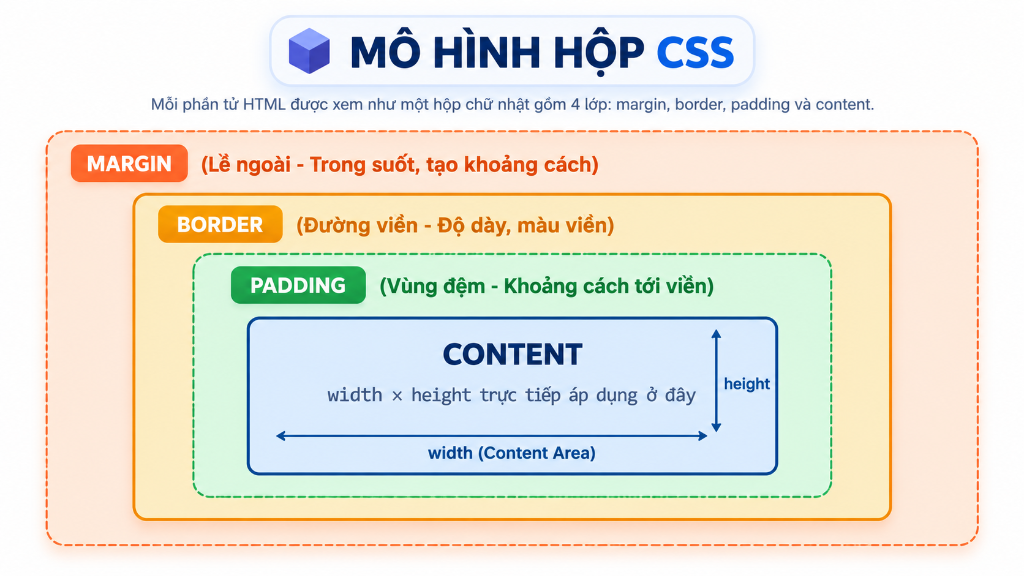
\includegraphics[width=0.82\linewidth]{figures/css_box_model_four_layers.png}
\caption{Sơ Đồ Trực Quan Hóa Mô Hình Hộp CSS (CSS Box Model) Với 4 Phân Tầng: Margin, Border, Padding Và Content}
\label{fig:css_box_model_four_layers}
\end{figure}

% ------------------------------------------------------------------------------
% 2.2 THUỘC TÍNH BOX-SIZING
% ------------------------------------------------------------------------------
\subsection{Thuộc Tính \csshint{box-sizing} (Thay Đổi Cách Tính Toán Kích Thước)}
\label{subsec:box_sizing_deep_dive}

Đây là thuộc tính quan trọng nhất ảnh hưởng trực tiếp đến cách trình duyệt tính toán \codeinline{width} và \codeinline{height} thực tế của phần tử trên trang.

\subsubsection{Mô Thức 1: \csshint{box-sizing: content-box;} (Mặc Định Chuẩn W3C)}

\begin{itemize}[leftmargin=1.5em, itemsep=3pt, parsep=0pt]
    \item \codeinline{width} và \codeinline{height} chỉ bao gồm kích thước của \textbf{Content Area (Vùng nội dung)}.
    \item \codeinline{padding} và \codeinline{border} sẽ được \textbf{cộng thêm vào bên ngoài} kích thước đã đặt của \codeinline{width} và \codeinline{height}.
    \item \textbf{Ví dụ tính toán thực tế}: Nếu bạn có một thẻ \codeinline{<div>} với:
    \begin{itemize}[leftmargin=1.2em, itemsep=2pt, parsep=0pt]
        \item Khai báo: \codeinline{width: 200px; padding: 10px; border: 2px solid;}
        \item Chiều rộng nội dung là: $200\text{px}$.
        \item Chiều rộng thực tế mà phần tử chiếm trên trang (\term{layout width}) sẽ là:
        \[
        \text{Layout Width} = 200\text{px (content)} + 10\text{px (left pad)} + 10\text{px (right pad)} + 2\text{px (left bor)} + 2\text{px (right bor)} = \mathbf{224\text{px}}
        \]
    \end{itemize}
\end{itemize}

\subsubsection{Mô Thức 2: \csshint{box-sizing: border-box;} (Rất Được Khuyến Nghị)}

\begin{itemize}[leftmargin=1.5em, itemsep=3pt, parsep=0pt]
    \item \codeinline{width} và \codeinline{height} bao gồm toàn bộ kích thước của \textbf{Content Area + Padding + Border}.
    \item \codeinline{padding} và \codeinline{border} sẽ được \textbf{tính gộp vào bên trong} kích thước \codeinline{width} và \codeinline{height} đã đặt. Vùng nội dung (Content Area) sẽ tự động co lại để nhường chỗ cho \codeinline{padding} và \codeinline{border}.
    \item \textbf{Ví dụ tính toán thực tế}: Nếu bạn có một thẻ \codeinline{<div>} với:
    \begin{itemize}[leftmargin=1.2em, itemsep=2pt, parsep=0pt]
        \item Khai báo: \codeinline{width: 200px; padding: 10px; border: 2px solid; box-sizing: border-box;}
        \item Chiều rộng thực tế mà phần tử chiếm trên trang (\term{layout width}) sẽ là: đúng $\mathbf{200\text{px}}$.
        \item Chiều rộng nội dung còn lại sẽ là:
        \[
        \text{Content Width} = 200\text{px} - (10\text{px} \times 2)\text{ (padding)} - (2\text{px} \times 2)\text{ (border)} = \mathbf{176\text{px}}
        \]
    \end{itemize}
    \item \textbf{Lợi ích vượt trội}: Điều này giúp việc tính toán bố cục dễ dàng và trực quan hơn rất nhiều, vì tổng kích thước của phần tử luôn luôn đúng với con số \codeinline{width} và \codeinline{height} mà bạn đã đặt trong mã nguồn. Đây là lý do tại sao nhiều khung làm việc (\term{framework}) CSS như Bootstrap, TailwindCSS và mọi dự án web hiện đại đều đặt \codeinline{box-sizing: border-box;} cho tất cả các phần tử (thường là với bộ chọn toàn cục \codeinline{* \{ box-sizing: border-box; \}}).
\end{itemize}

\begin{figure}[H]
\centering
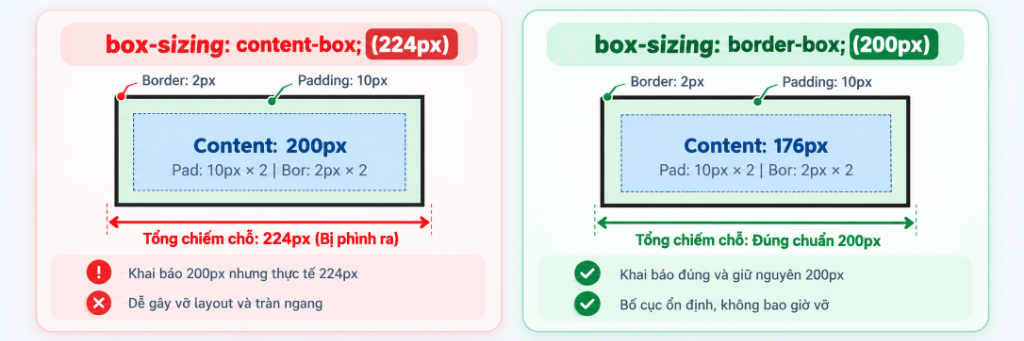
\includegraphics[width=\linewidth]{figures/box_sizing_content_vs_border_box.png}
\caption{So Sánh Cơ Chế Chiếm Chỗ: \codeinline{content-box} (Phình To Ra 224px) vs \codeinline{border-box} (Bảo Toàn Kích Thước 200px)}
\label{fig:box_sizing_content_vs_border_box}
\end{figure}

% ==============================================================================
% MỤC 3: LƯU Ý CHI TIẾT KHI SỬ DỤNG WIDTH VÀ HEIGHT
% ==============================================================================
\section{Lưu Ý Chi Tiết Khi Sử Dụng \csshint{width} \& \csshint{height}}
\label{sec:detailed_width_height_caveats}

Trong quá trình xây dựng giao diện thực tế, việc sử dụng \codeinline{width} và \codeinline{height} có thể dẫn đến nhiều lỗi hiển thị khó lường nếu không nắm chắc 5 nguyên lý cơ bản sau đây.

% ------------------------------------------------------------------------------
% 3.1 GIÁ TRỊ AUTO VÀ HÀNH VI KHÁC BIỆT
% ------------------------------------------------------------------------------
\subsection{Giá Trị auto – Bản Chất Bất Đối Xứng Và Cơ Chế Kích Thước Tự Động}
\label{subsec:auto_behavior_by_display}

Trong CSS, \codeinline{auto} là một từ khóa đặc biệt mang tính quyết định đến cách thức bố cục vận hành. Thiết lập \codeinline{width: auto;} hoặc \codeinline{height: auto;} (hoặc hoàn toàn \textbf{không khai báo} kích thước) đồng nghĩa với việc bạn chuyển giao toàn bộ quyền tính toán kích thước cho thuật toán phân bổ không gian (\term{Normal Flow Algorithm}) của trình duyệt.

Thuật toán này sẽ tính toán kích thước dựa trên 4 yếu tố ngữ cảnh cốt lõi:
\begin{enumerate}[leftmargin=1.5em, itemsep=2.5pt, parsep=0pt]
    \item \textbf{Loại phần tử}: Phần tử khối (\term{block-level}), phần tử nội dòng (\term{inline-level}), hay phần tử thay thế (\term{replaced element} như \codeinline{<img>}).
    \item \textbf{Nội dung bên trong}: Chiều dài văn bản, số lượng dòng chữ, hoặc kích thước pixel tự nhiên (\term{intrinsic size}) của tệp đa phương tiện.
    \item \textbf{Không gian khả dụng của phần tử cha}: Chiều rộng khả dụng của khung chứa hoặc các ràng buộc bố cục nâng cao (\codeinline{flex}, \codeinline{grid}).
    \item \textbf{Mô hình hộp và các thuộc tính kiểm soát}: Tác động trực tiếp từ \codeinline{box-sizing}, \codeinline{padding}, \codeinline{border}, \codeinline{min-*}, \codeinline{max-*}.
\end{enumerate}

\begin{figure}[H]
\centering
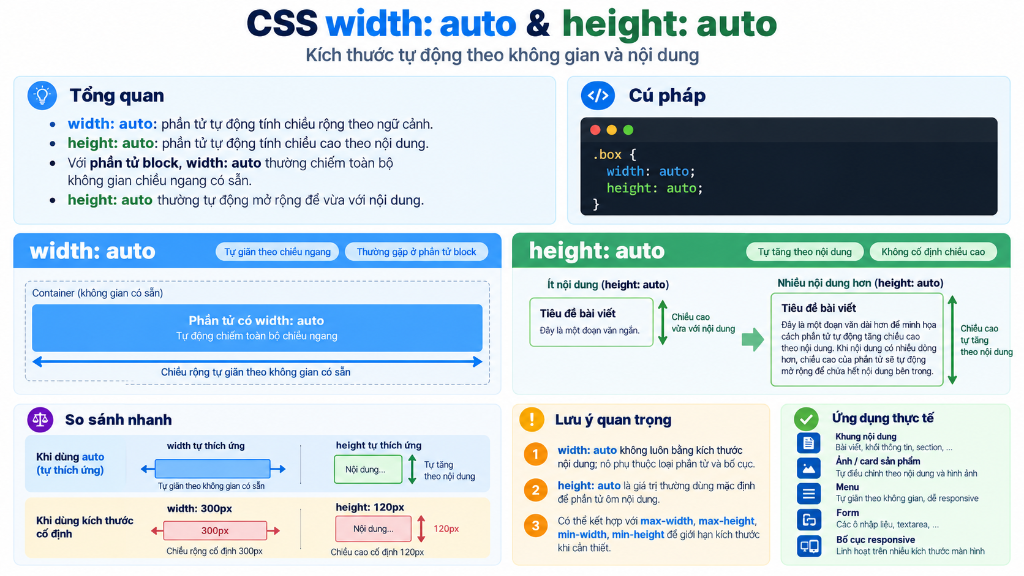
\includegraphics[width=\linewidth]{figures/css_auto_dimensions_overview.png}
\caption{Infographic Tổng Quan: Cơ Chế Tự Động Tính Toán Kích Thước Của \codeinline{width: auto;} \& \codeinline{height: auto;}}
\label{fig:css_auto_dimensions_overview}
\end{figure}

\begin{conceptBox}[Khái Niệm Cốt Lõi: Bản Chất Bất Đối Xứng Của Giá Trị auto Giữa Hai Trục]
Nhiều lập trình viên mới học thường thắc mắc: \textit{``Tại sao \codeinline{width: auto;} lại tự động bung trọn khung chứa, trong khi \codeinline{height: auto;} lại co cụm ôm sát nội dung?''}\\
Câu trả lời nằm ở \textbf{nguyên lý dòng chảy tự nhiên của tài liệu web}:
\begin{itemize}[leftmargin=1.2em, itemsep=2.5pt, parsep=0pt]
    \item \textbf{Trục ngang (Inline Axis)} có giới hạn vật lý nghiêm ngặt bởi khung nhìn thiết bị (viewport). Để thuận tiện cho việc trình bày văn bản theo dòng, các phần tử khối mặc định có tính chất ``thèm khát không gian ngang'' (\term{greedy width}) --- tự động bung ra chiếm $100\%$ không gian cha để chứa được nhiều chữ nhất trên mỗi dòng.
    \item \textbf{Trục dọc (Block Axis)} của trang web có độ dài vô hạn thông qua thao tác cuộn chuột. Nếu phần tử cũng tự động bung $100\%$ chiều cao cha, các khối phía sau sẽ bị đẩy rơi xuống đáy, tạo ra các khoảng trống khổng lồ vô nghĩa. Vì vậy, \codeinline{height: auto;} được thiết kế mang tính chất ``tiết kiệm không gian dọc'' --- chỉ mở rộng vừa đủ để chứa trọn lượng nội dung con bên trong.
\end{itemize}
\end{conceptBox}

\subsubsection{a) Đối Với \csshint{width: auto;} \& Cuộc Chạm Trán Với \csshint{width: 100\%;}}

Khi áp dụng \codeinline{width: auto;}, hành vi sẽ phân hóa rõ rệt tùy theo chế độ hiển thị:
\begin{itemize}[leftmargin=1.5em, itemsep=3.5pt, parsep=0pt]
    \item \textbf{Phần tử khối (\term{Block-level elements}, ví dụ \codeinline{<div>}, \codeinline{<p>}, \codeinline{<section>})}:
    Tự động chiếm toàn bộ chiều rộng có sẵn trong phần tử cha (trừ đi margin, padding, border của chính nó).
    \item \textbf{Phần tử nội dòng (\term{Inline-level elements}, ví dụ \codeinline{<span>}, \codeinline{<a>}, \codeinline{<strong>})}:
    \textbf{Hoàn toàn phớt lờ} mọi khai báo \codeinline{width} cố định. Kích thước bề ngang chỉ bằng đúng độ dài chuỗi ký tự hoặc hình ảnh nội dòng bên trong.
    \item \textbf{Phần tử nội dòng khối (\codeinline{inline-block}) hoặc Phần tử trôi nổi (\codeinline{float})}:
    Tự động co lại ôm sát nội dung (\term{shrink-wrap}), chỉ mở rộng khi nội dung bên trong dài thêm.
\end{itemize}

\begin{noteBox}[Giải Mã Cốt Lõi: So Sánh width: auto vs width: 100\% \& Tác Động Của box-sizing]
Đây là điểm gây hiểu lầm và lỗi vỡ bố cục phổ biến nhất trong xây dựng giao diện CSS:
\begin{itemize}[leftmargin=1.2em, itemsep=3pt, parsep=0pt]
    \item \textbf{Khi dùng \codeinline{width: auto;}}: Trình duyệt tự giải phương trình kích thước thông minh:
    $$\text{Chiều Rộng Nội Dung} = \text{Chiều Rộng Cha} - (\text{Margin} + \text{Padding} + \text{Border})$$
    Nhờ cơ chế tự bù trừ này, phần tử \textbf{KHÔNG BAO GIỜ bị tràn khung cha}, ngay cả khi dự án chưa thiết lập \codeinline{box-sizing: border-box;}.
    \item \textbf{Khi dùng \codeinline{width: 100\%;}}: Bạn đang ép bề ngang vùng đệm (\term{content area}) bằng chính xác $100\%$ không gian cha. Nếu sau đó bạn thêm \codeinline{padding: 20px;} hoặc \codeinline{border: 5px;}, tổng bề ngang thực tế sẽ bằng $100\% + 50\text{px}$, dẫn đến việc \textbf{hộp bị phình to vỡ tràn ra ngoài khung chứa}, sinh ra thanh cuộn ngang gây lỗi giao diện nghiêm trọng!
\end{itemize}
\end{noteBox}

\subsubsection{b) Đối Với \csshint{height: auto;} \& Cơ Chế Khi Không Khai Báo height}

Khi lập trình viên \textbf{không khai báo \codeinline{height}}, trình duyệt sẽ tự động mặc định áp dụng \codeinline{height: auto;}. Cơ chế vận hành cụ thể gồm 4 kịch bản liên kết chặt chẽ:
\begin{enumerate}[leftmargin=1.5em, itemsep=3.5pt, parsep=0pt]
    \item \textbf{Kịch bản 1: Nội dung rỗng \& không có padding}: Chiều cao phần tử sụp đổ về đúng $0\text{px}$. Khối hộp hoàn toàn vô hình trên trang dù bạn có tô màu nền bắt mắt.
    \item \textbf{Kịch bản 2: Có nội dung văn bản/con}: Chiều cao co giãn mềm dẻo và tự thích ứng với số lượng dòng chữ (1 dòng thì mỏng, nhiều dòng thì đáy hộp tự động đẩy sâu xuống).
    \item \textbf{Kịch bản 3: Tác động của padding khi không có height}: Chiều cao luôn được bảo toàn tối thiểu bằng $\text{padding-top} + \text{padding-bottom}$. Một khối rỗng chữ nhưng có \codeinline{padding: 20px;} vẫn sẽ hiển thị một khối màu chữ nhật dày $40\text{px}$ rõ ràng.
    \item \textbf{Kịch bản 4: Khi nào chiều cao KHÔNG bằng chiều cao nội dung?}:
    \begin{itemize}[leftmargin=1.2em, itemsep=2pt, parsep=0pt]
        \item \textbf{Khi có \codeinline{height} cố định}: Bị đóng băng kích thước; nếu nội dung dài hơn sẽ bị tràn (\term{overflow}).
        \item \textbf{Khi có \codeinline{min-height}}: Đóng vai trò \textbf{chốt chặn sàn} an toàn, đảm bảo giao diện không bị co rúm xẹp lép khi dữ liệu chưa tải về kịp từ máy chủ.
        \item \textbf{Khi có \codeinline{max-height}}: Đóng vai trò \textbf{chốt chặn trần}, ngăn phần tử kéo dài vô tận làm hỏng cấu trúc trang; khi vượt ngưỡng sẽ kích hoạt thanh cuộn dọc nếu đi kèm \codeinline{overflow-y: auto;}.
    \end{itemize}
\end{enumerate}

\begin{figure}[H]
\centering
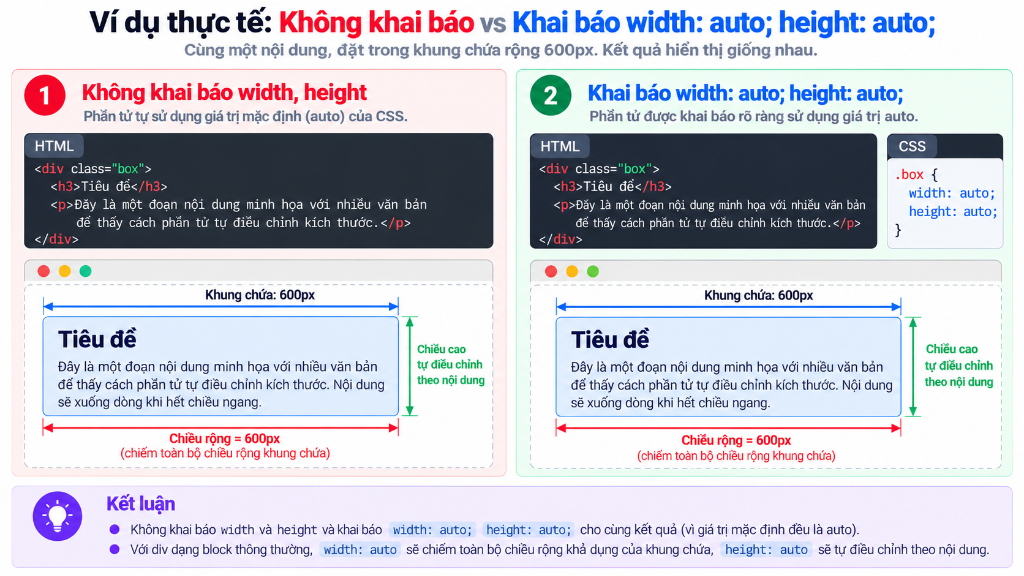
\includegraphics[width=\linewidth]{figures/css_auto_vs_undeclared_box_comparison.png}
\caption{Thực Nghiệm Bố Cục: Không Khai Báo vs Khai Báo \codeinline{width: auto; height: auto;} Cho Cùng Kết Quả Trong Khung Chứa 600px}
\label{fig:css_auto_vs_undeclared_box_comparison}
\end{figure}

\begin{figure}[H]
\centering
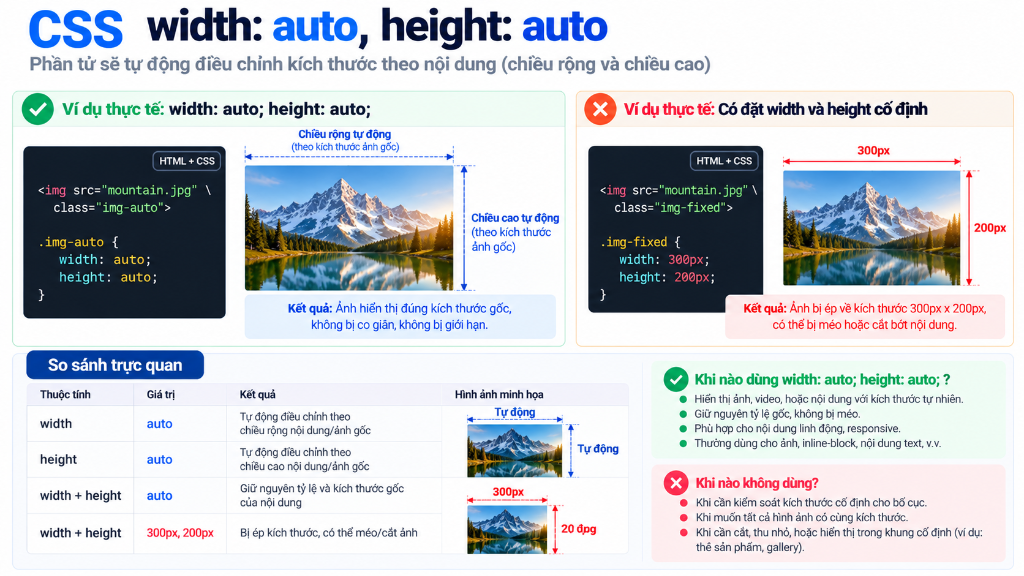
\includegraphics[width=\linewidth]{figures/css_auto_vs_fixed_image_comparison.png}
\caption{Đối Chiếu Trực Quan: \codeinline{width: auto; height: auto;} Bảo Toàn Kích Thước Gốc vs Kích Thước Cố Định Làm Méo Ảnh}
\label{fig:css_auto_vs_fixed_image_comparison}
\end{figure}

\begin{warnBox}[Cạm Bẫy Kinh Điển: Thuộc Tính height: 100\% Bị Liệt Trên Cha auto!]
Một phần tử con khai báo \codeinline{height: 100\%;} sẽ \textbf{chỉ hoạt động nếu phần tử cha có chiều cao tường minh bằng con số cụ thể} (ví dụ: \codeinline{height: 400px;} hoặc \codeinline{height: 100vh;}).\\
Nếu phần tử cha đang để mặc định \codeinline{height: auto;}, trình duyệt rơi vào vòng lặp vô định: \textit{Con đòi $100\%$ của Cha, nhưng Cha lại đợi Con nở ra mới biết mình cao bao nhiêu}. Kết quả: Trình duyệt hủy bỏ lệnh \codeinline{height: 100\%;} và con tự teo lại theo nội dung của nó!
\end{warnBox}

\begin{codeWindow}[Ví Dụ Sửa Cạm Bẫy height: 100\%]
\begin{lstlisting}[language=HTML5, escapeinside={(*@}{@*)}]
<!-- TRUONG HOP LOI: .child khong the dat 100% vi .parent la auto -->
<div class="parent" style="height: auto;">
    <div class="child" style="height: 100%; background: lightcoral;">
        (*@Con bi teo lai vi cha khong co chieu cao xac dinh!@*)
    </div>
</div>

<!-- GIAI PHAP CHUAN: Xac dinh chieu cao cho cha hoac dung viewport unit -->
<div class="parent-fixed" style="height: 300px;">
    <div class="child" style="height: 100%; background: lightgreen;">
        (*@Con nhan du 100% cua 300px = 300px hoan hao!@*)
    </div>
</div>
\end{lstlisting}
\end{codeWindow}

\begin{tipBox}[Góc Đọc Thêm: Vì Sao auto Trên Thẻ img Lại Khác Với Thẻ div?]
Nhiều bạn đọc tinh ý sẽ nhận ra: Tại sao ở Hình~\ref{fig:css_auto_dimensions_overview}, thẻ \codeinline{<div>} có \codeinline{width: auto;} lại bung $100\%$ màn hình; nhưng ở Hình~\ref{fig:css_auto_vs_fixed_image_comparison}, thẻ \codeinline{<img>} có \codeinline{width: auto;} lại giữ đúng $1200\text{px}$ của ảnh gốc mà không bung theo khung chứa?\\
\textbf{Bí mật nằm ở sự khác biệt giữa hai nhóm phần tử}:
\begin{itemize}[leftmargin=1.2em, itemsep=2.5pt, parsep=0pt]
    \item Thẻ \codeinline{<div>}, \codeinline{<p>} là \textbf{phần tử không thay thế} (\term{non-replaced elements}): Bản thân chúng là các khung chứa cấu trúc rỗng, kích thước bề ngang hoàn toàn do thuật toán dòng chảy văn bản quy định.
    \item Thẻ \codeinline{<img>}, \codeinline{<video>} là \textbf{phần tử thay thế} (\term{replaced elements}): Nội dung của chúng được tải từ tệp ngoài. Bản thân tệp ảnh đã sở hữu \textbf{kích thước tự nhiên} (\term{intrinsic width/height}) và \textbf{tỷ lệ khung hình} (\term{intrinsic aspect ratio}). Khi đặt \codeinline{width: auto; height: auto;}, trình duyệt diễn giải là: \textit{``Hãy hiển thị trung thực đúng kích thước gốc của bức ảnh''}.
    \item Vì vậy, nếu tệp ảnh gốc rộng tới $1200\text{px}$, nó sẽ đâm toang khung chứa $600\text{px}$! Đây chính là lý do vì sao công thức responsive bất hủ \codeinline{max-width: 100\%; height: auto;} ra đời (sẽ được phân tích chi tiết tại Mục~\ref{subsec:min_max_sizing}).
\end{itemize}
\end{tipBox}

\begin{prettyTableBox}[Ma Trận Tổng Hợp: So Sánh Bản Chất Các Thuộc Tính Đo Lường Cơ Bản]
\rowcolors{2}{white}{primaryBlue!4}
\begin{tabularx}{\linewidth}{>{\bfseries\color{primaryBlue}}L{2.5cm} C{2.2cm} Z Z}
\rowcolor{primaryBlue}
\thd{Thuộc Tính} & \thd{Giá Trị Mặc Định} & \thd{Cơ Chế Tính Toán Của Trình Duyệt} & \thd{Lời Khuyên Kiến Trúc Frontend} \\
\codeinline{width: auto} & Mặc định thẻ HTML & Block: chiếm trọn 100\% ngang cha. Inline: vừa khít chữ. Replaced: lấy ảnh gốc. & Dùng cho cấu trúc layout linh hoạt, tự thích ứng với padding/border. \\
\codeinline{width: 100\%} & Tự định nghĩa & Ép vùng đệm nội dung bằng đúng 100\% cha. Dễ tràn khung nếu thiếu border-box. & Chỉ dùng khi cần ép rộng, luôn đi kèm \codeinline{box-sizing: border-box}. \\
\codeinline{height: auto} & Mặc định thẻ HTML & Co dãn theo nội dung con. Bằng 0 nếu rỗng và không có padding. & Luôn là lựa chọn hàng đầu cho văn bản để tránh lỗi tràn chữ khi responsive. \\
\codeinline{min-height} & \codeinline{0} (hoặc auto) & Tạo ngưỡng sàn tối thiểu, cho phép nở cao hơn nếu nội dung vượt mức. & Dùng cho Card sản phẩm, Hero section để chống thụt xẹp giao diện. \\
\codeinline{max-height} & \codeinline{none} & Tạo ngưỡng trần tối đa, thường kết hợp \codeinline{overflow-y: auto}. & Dùng cho Modal pop-up, danh sách bình luận, khung chat box. \\
\end{tabularx}
\end{prettyTableBox}

% ------------------------------------------------------------------------------
% 3.2 ĐƠN VỊ TƯƠNG ĐỐI VÀ TUYỆT ĐỐI
% ------------------------------------------------------------------------------
\subsection{Đơn Vị Tương Đối Và Đơn Vị Tuyệt Đối}
\label{subsec:units_relative_vs_absolute}

\subsubsection{a) Đơn Vị Tuyệt Đối (Absolute Units): \csshint{px}, \csshint{pt}, \csshint{cm}, \csshint{in}...}
\begin{itemize}[leftmargin=1.5em, itemsep=3pt, parsep=0pt]
    \item Cố định, không thay đổi theo kích thước màn hình thiết bị hay kích cỡ phông chữ của người dùng.
    \item \textbf{Lưu ý thực chiến}: Việc lạm dụng và sử dụng \codeinline{px} quá nhiều cho \codeinline{width} và \codeinline{height} của các container lớn có thể làm cho trang web trở nên cứng nhắc, kém linh hoạt và cực kỳ khó khăn khi chuyển đổi giao diện đáp ứng (\term{responsive}) trên màn hình điện thoại di động hoặc máy tính bảng.
\end{itemize}

\subsubsection{b) Đơn Vị Tương Đối (Relative Units): \csshint{\%}, \csshint{em}, \csshint{rem}, \csshint{vw}, \csshint{vh}...}
\begin{itemize}[leftmargin=1.5em, itemsep=4pt, parsep=0pt]
    \item \textbf{\codeinline{\%} (Phần trăm)}: Luôn luôn tương đối so với kích thước của phần tử cha trực tiếp. Nếu phần tử cha không có kích thước rõ ràng hoặc đang để \codeinline{height: auto;}, đơn vị \codeinline{\%} có thể không hoạt động như mong đợi.
    \item \textbf{\codeinline{em}}: Tương đối so với \codeinline{font-size} của chính phần tử đó (hoặc của phần tử cha nếu \codeinline{font-size} không được định nghĩa trên chính nó). Rất hữu ích cho các thành phần UI có kích thước tỷ lệ thuận với văn bản (ví dụ: nút bấm có \codeinline{padding} và \codeinline{width} giãn nở nhịp nhàng theo cỡ chữ).
    \item \textbf{\codeinline{rem}}: Tương đối so với \codeinline{font-size} của phần tử gốc \codeinline{<html>}. Giúp duy trì tỷ lệ kích thước hài hòa và đồng nhất trên toàn bộ hệ thống trang web.
    \item \textbf{\codeinline{vw} (\term{Viewport Width}) / \codeinline{vh} (\term{Viewport Height})}: Tương đối so với kích thước thực của cửa sổ trình duyệt (\term{viewport}). $1\text{vw}$ là $1\%$ chiều rộng viewport, $1\text{vh}$ là $1\%$ chiều cao viewport. Đây là lựa chọn tuyệt vời cho các phần tử cần chiếm một tỷ lệ cố định của màn hình thiết bị, ví dụ: \codeinline{height: 100vh;} để tạo một \term{Hero Section} tràn đầy trọn vẹn màn hình mở đầu.
    \item \textbf{Lưu ý}: Các đơn vị tương đối giúp tạo ra thiết kế linh hoạt, co giãn mượt mà và đáp ứng tốt hơn trên mọi thiết bị hiện đại.
\end{itemize}

% ------------------------------------------------------------------------------
% 3.3 MIN/MAX WIDTH & HEIGHT
% ------------------------------------------------------------------------------
\subsection{Kiểm Soát Giới Hạn: \csshint{min-width}, \csshint{max-width}, \csshint{min-height}, \csshint{max-height}}
\label{subsec:min_max_sizing}

Đây là nhóm bốn thuộc tính cực kỳ quan trọng và không thể thiếu trong kỹ thuật thiết kế giao diện đáp ứng (\term{Responsive Web Design}):

\begin{enumerate}[leftmargin=1.5em, itemsep=6pt, parsep=0pt]
    \item \textbf{\codeinline{max-width: 100\%;} (Quy chuẩn vàng tối thượng cho hình ảnh)}:
    \begin{itemize}[leftmargin=1.2em, itemsep=2pt, parsep=0pt]
        \item Giúp hình ảnh không bao giờ tràn ra khỏi vùng chứa của nó, tự động co lại một cách linh hoạt khi màn hình thu hẹp hơn kích thước gốc của ảnh.
        \item Khối quy tắc kinh điển mà mọi lập trình viên Frontend đều phải thuộc lòng:
        \begin{codeWindow}[Bộ Quy Tắc Ảnh Responsive Chuẩn Công Nghiệp]
\begin{lstlisting}[language=CSS3]
img {
    max-width: 100%;
    height: auto;
    display: block;
}
\end{lstlisting}
        \end{codeWindow}
        \item Thuộc tính \codeinline{height: auto;} đi kèm đảm bảo tỷ lệ khung hình (\term{aspect ratio}) của bức ảnh được bảo toàn nguyên vẹn, không bao giờ bị méo mó hình ảnh.
    \end{itemize}

    \item \textbf{Cặp Thuộc Tính Chốt Chặn Sàn: \codeinline{min-width} Và \codeinline{min-height}}:
    
    \codeinline{min-width} và \codeinline{min-height} là hai thuộc tính CSS chuyên dụng giúp thiết lập \textbf{giới hạn tối thiểu} cho kích thước của một phần tử:
    \begin{itemize}[leftmargin=1.2em, itemsep=2.5pt, parsep=0pt]
        \item \codeinline{min-width}: Xác định chiều rộng nhỏ nhất cho phép. Phần tử tuyệt đối không được co nhỏ hơn giá trị này. Nếu nội dung bên trong đòi hỏi không gian lớn hơn, phần tử sẽ tự do mở rộng ra ngoài.
        \item \codeinline{min-height}: Xác định chiều cao nhỏ nhất cho phép. Phần tử tuyệt đối không được thấp hơn giá trị này. Khi nội dung con phát triển nhiều dòng hơn, phần tử sẽ tự động giãn cao theo nội dung.
    \end{itemize}

    \begin{figure}[H]
    \centering
    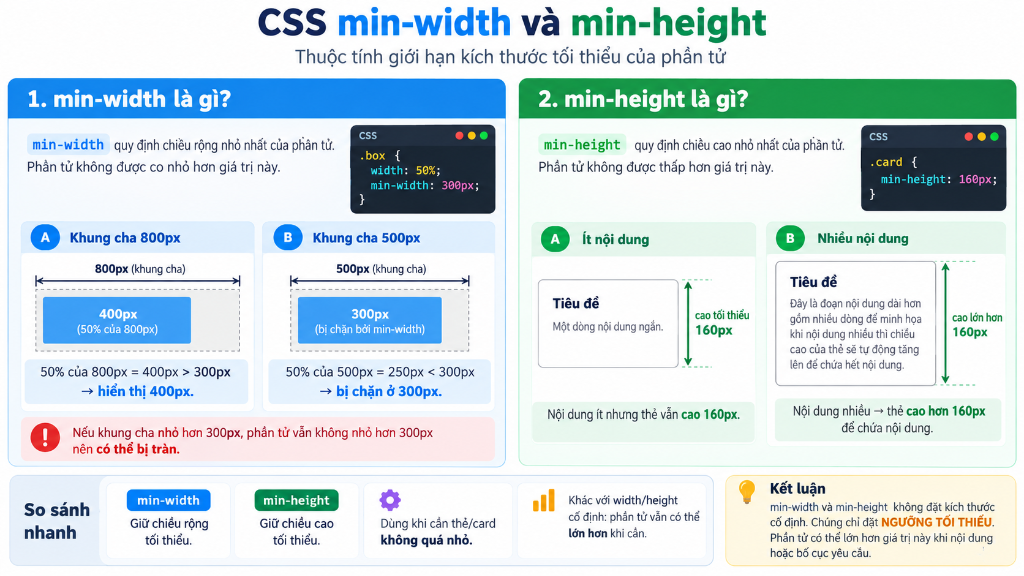
\includegraphics[width=\linewidth]{figures/css_min_width_min_height_overview.png}
    \caption{Infographic Toàn Cảnh: Cơ Chế Giới Hạn Kích Thước Tối Thiểu Của \codeinline{min-width} \& \codeinline{min-height}}
    \label{fig:css_min_width_min_height_overview}
    \end{figure}

    \paragraph{a) Cách hoạt động của \codeinline{min-width} \& Thí nghiệm thực chứng DevTools:}
    Xét một ví dụ kinh điển trong đó \codeinline{width} cố định xung đột trực tiếp với \codeinline{min-width}:
    \begin{codeWindow}[Thực Nghiệm min-width Đè Bẹp width Cố Định]
\begin{lstlisting}[language=HTML5, escapeinside={(*@}{@*)}]
<style>
.box {
    background: lightblue;
    min-width: 300px;
    width: 100px; /* Khong co tac dung vi nho hon min-width! */
}
</style>
<div class="box">Noi dung BOX</div>
\end{lstlisting}
    \end{codeWindow}

    \textbf{Kiểm chứng thực tế trên Chrome DevTools}:
    \begin{itemize}[leftmargin=1.2em, itemsep=3pt, parsep=0pt]
        \item \textbf{Khi nội dung ngắn}: Dù lập trình viên đã viết \codeinline{width: 100px;}, nhưng cửa sổ Inspect của trình duyệt vẫn hiển thị chính xác kích thước hộp là $\mathbf{300 \times 17.6\text{px}}$ (Hình~\ref{fig:devtools_min_width_override}). Giá trị \codeinline{min-width: 300px;} đã hoàn toàn áp đảo và đè bẹp khai báo \codeinline{width: 100px;}.
        \item \textbf{Khi nội dung dài hơn}: Nếu ta thay đổi nội dung thành chuỗi văn bản dài: \codeinline{<div class="box">Nếu nội dung nhiều hơn thì box giản ra theo nội dung</div>}, văn bản sẽ tự động rớt xuống 2 dòng, chiều cao tăng vọt từ $17.6\text{px}$ lên $\mathbf{35.2\text{px}}$ (Hình~\ref{fig:devtools_min_width_expand_height}), trong khi bề ngang vẫn được bảo toàn nguyên vẹn ở mức $300\text{px}$.
    \end{itemize}

    \begin{figure}[H]
    \centering
    \begin{minipage}{0.48\linewidth}
        \centering
        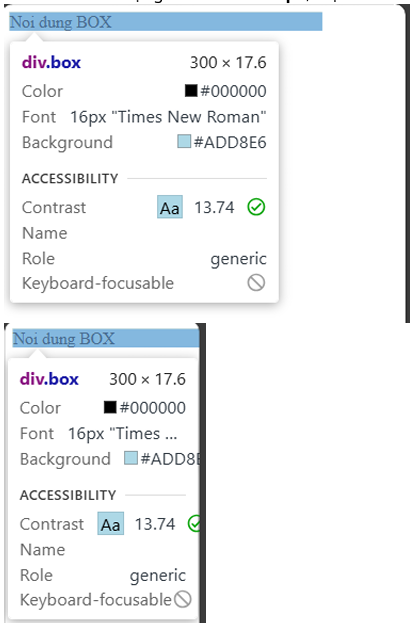
\includegraphics[width=0.88\linewidth]{figures/devtools_min_width_override.png}
        \caption{DevTools: \codeinline{min-width: 300px} Đè Bẹp \codeinline{width: 100px}}
        \label{fig:devtools_min_width_override}
    \end{minipage}\hfill
    \begin{minipage}{0.48\linewidth}
        \centering
        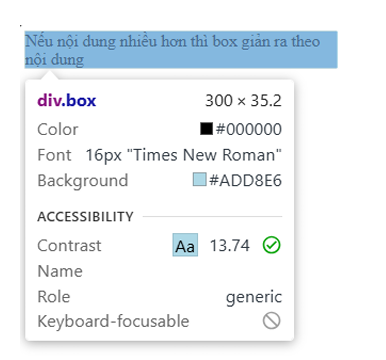
\includegraphics[width=0.88\linewidth]{figures/devtools_min_width_expand_height.png}
        \caption{DevTools: Khi Thêm Chữ, Chiều Cao Tự Nở Ra Đạt $35.2\text{px}$}
        \label{fig:devtools_min_width_expand_height}
    \end{minipage}
    \end{figure}

    \textbf{Cơ chế khi kết hợp \codeinline{min-width} với đơn vị phần trăm (\%)}:\\
    Khi ta thiết lập \codeinline{.box \{ width: 50\%; min-width: 300px; \}}:
    \begin{itemize}[leftmargin=1.2em, itemsep=2pt, parsep=0pt]
        \item \textbf{Trong khung cha $800\text{px}$}: Chiều rộng tính toán là $50\% \times 800\text{px} = 400\text{px} > 300\text{px} \rightarrow$ Hiển thị $400\text{px}$.
        \item \textbf{Trong khung cha $500\text{px}$}: Chiều rộng tính toán là $50\% \times 500\text{px} = 250\text{px} < 300\text{px} \rightarrow$ Bị chốt chặn dừng lại ở $300\text{px}$.
        \item \textbf{Lưu ý rủi ro}: Nếu khung cha nhỏ hơn $300\text{px}$ (ví dụ màn hình di động hẹp), phần tử sẽ không thể thu nhỏ hơn $300\text{px}$ nữa và sẽ \textbf{bị tràn khung ngang}.
    \end{itemize}

    \paragraph{b) Cách hoạt động của \codeinline{min-height}:}
    Tương tự như chiều rộng, \codeinline{min-height} giải quyết bài toán chống sụp xẹp giao diện:
    \begin{codeWindow}[Ví Dụ min-height Bảo Toàn Chiều Cao Tối Thiểu]
\begin{lstlisting}[language=HTML5, escapeinside={(*@}{@*)}]
.box {
    background: lightgreen;
    min-height: 200px;
    height: 50px; /* Bi vo hieu hoa boi min-height! */
}
\end{lstlisting}
    \end{codeWindow}
    \begin{itemize}[leftmargin=1.2em, itemsep=2.5pt, parsep=0pt]
        \item Khi phần tử có ít chữ: Khối vẫn đứng sừng sững với chiều cao $200\text{px}$, giữ vững bố cục lưới (\term{Grid/Flex card}) không bị chênh lệch so với các thẻ lân cận.
        \item Khi phần tử nhận nhiều dữ liệu từ API: Chiều cao tự động bung lớn hơn $200\text{px}$ để bao trọn toàn bộ nội dung, không bao giờ xảy ra tình trạng cắt cụt chữ.
    \end{itemize}

    \paragraph{c) Nghệ thuật kết hợp 4 cực kích thước: \codeinline{min-width}, \codeinline{max-width}, \codeinline{min-height}, \codeinline{max-height}:}
    Bằng cách kết hợp đồng thời cả 4 thuộc tính giới hạn, lập trình viên tạo ra một \textbf{hộp co giãn trong dải an toàn tuyệt đối}:
    \begin{codeWindow}[Hộp Kích Thước Co Giãn Trong Khoảng An Toàn]
\begin{lstlisting}[language=CSS3]
.box {
    background: orange;
    min-width: 200px;
    max-width: 400px;
    min-height: 150px;
    max-height: 300px;
    overflow: auto;
}
\end{lstlisting}
    \end{codeWindow}
    \begin{itemize}[leftmargin=1.2em, itemsep=2pt, parsep=0pt]
        \item Bề ngang dao động an toàn trong dải $[200\text{px}, 400\text{px}]$.
        \item Bề dọc dao động an toàn trong dải $[150\text{px}, 300\text{px}]$; nếu nội dung vượt trần $300\text{px}$, thanh cuộn nội bộ tự động xuất hiện nhờ \codeinline{overflow: auto;}.
    \end{itemize}

    \begin{prettyTableBox}[Ma Trận 4 Thuộc Tính Ranh Giới Kích Thước Trong CSS]
    \rowcolors{2}{white}{primaryBlue!4}
    \begin{tabularx}{\linewidth}{>{\bfseries\color{primaryBlue}}L{2.5cm} Z Z}
    \rowcolor{primaryBlue}
    \thd{Thuộc Tính} & \thd{Ý Nghĩa Ranh Giới} & \thd{Ứng Dụng Thực Chiến} \\
    \codeinline{min-width} & Đảm bảo phần tử không bao giờ nhỏ hơn giá trị này. & Bảo vệ nút bấm, thẻ Card, Sidebar không bị thu nhỏ quá mức trên mobile. \\
    \codeinline{min-height} & Đảm bảo phần tử không bao giờ thấp hơn giá trị này. & Giữ thẻ Card sản phẩm bằng nhau, chống xẹp khung khi dữ liệu chưa load. \\
    \codeinline{max-width} & Đảm bảo phần tử không bao giờ lớn hơn giá trị này. & Giữ độ dài dòng đọc lý tưởng, chống tràn ảnh responsive (\codeinline{max-width: 100\%}). \\
    \codeinline{max-height} & Đảm bảo phần tử không bao giờ cao hơn giá trị này. & Khóa trần hộp chat, danh sách bình luận, popup modal kèm \codeinline{overflow: auto}. \\
    \end{tabularx}
    \end{prettyTableBox}

    \item \textbf{\codeinline{max-height}}:
    \begin{itemize}[leftmargin=1.2em, itemsep=2pt, parsep=0pt]
        \item Cực kỳ hữu ích khi bạn muốn giới hạn chiều cao tối đa của một khối nội dung để tránh nó kéo dài trang web quá mức (ví dụ: khung bình luận, danh sách thông báo, hộp thoại điều khoản).
        \item Thường được kết hợp với \codeinline{overflow-y: auto;} để sinh ra thanh cuộn dọc mượt mà khi lượng nội dung vượt quá giới hạn chiều cao cho phép.
        \item \textbf{Ví dụ}: \codeinline{max-height: 300px; overflow-y: auto;}.
    \end{itemize}
\end{enumerate}

\begin{tipBox}[Chiến Lược Thực Chiến Khi Sử Dụng min-width \& max-width]
\begin{itemize}[leftmargin=1.2em, itemsep=3pt, parsep=0pt]
    \item \textbf{Khóa biên dưới an toàn (\codeinline{min-width})}: Thiết lập cho các nút bấm hành động (button, input, badge) để tránh bị co rúm trên thiết bị di động màn hình hẹp ($< 360\text{px}$).
    \item \textbf{Khóa trần thị giác (\codeinline{max-width})}: Thiết lập cho các khối văn bản đọc (\codeinline{max-width: 700px} đến \codeinline{800px}) nhằm giữ độ dài dòng đọc ở mức lý tưởng (khoảng 60--75 ký tự/dòng theo chuẩn Ergonomics).
    \item \textbf{Cặp bài trùng Responsive}: Luôn ưu tiên công thức \codeinline{width: 100\%; max-width: 1200px; margin: 0 auto;} để tạo khối khung chứa trung tâm hoàn hảo cho mọi trang web.
\end{itemize}
\end{tipBox}

% ------------------------------------------------------------------------------
% 3.3.1 SỰ KẾT HỢP GIỮA MAX-WIDTH, MAX-HEIGHT VÀ WIDTH, HEIGHT
% ------------------------------------------------------------------------------
\subsubsection{Sự Kết Hợp Giữa max-width, max-height Và width, height: Quy Luật Hoạt Động \& Trạng Thái Vô Hiệu Hóa}
\label{subsubsec:combination_max_and_dimensions}

Trong thực tế xây dựng giao diện đáp ứng (\term{Responsive}), nhóm thuộc tính đo lường cơ bản (\codeinline{width}, \codeinline{height}) và nhóm giới hạn trần (\codeinline{max-width}, \codeinline{max-height}) thường xuyên được kết hợp với nhau. Tuy nhiên, nếu lập trình viên không hiểu rõ thứ tự ưu tiên của thuật toán CSS, các thuộc tính này có thể \textbf{triệt tiêu lẫn nhau} hoặc gây ra lỗi méo mó giao diện nghiêm trọng.

\paragraph{1. Bản Chất Đối Lập Giữa Kích Thước Cơ Sở Và Giới Hạn Trần:}
\begin{itemize}[leftmargin=1.5em, itemsep=3pt, parsep=0pt]
    \item \codeinline{width} / \codeinline{height}: Xác định kích thước cơ sở mà phần tử muốn đạt được (có thể là cố định bằng \codeinline{px} hoặc co giãn theo \codeinline{auto}/\codeinline{\%}).
    \item \codeinline{max-width} / \codeinline{max-height}: Thiết lập \textbf{ranh giới trần tuyệt đối}. Phần tử có thể co nhỏ hơn ngưỡng này, nhưng \textbf{tuyệt đối không bao giờ được phép vượt quá}.
\end{itemize}

\paragraph{2. Hai Trạng Thái Tương Tác Sống Còn:}
\begin{enumerate}[leftmargin=1.5em, itemsep=4pt, parsep=0pt]
    \item \textbf{Trạng thái 1: Khi \codeinline{max-width} hoặc \codeinline{max-height} hoạt động đúng hiệu lực}\\
    Bạn \textbf{không đặt kích thước cố định}, mà để kích thước tự do co giãn theo nội dung bằng cách sử dụng \codeinline{width: auto;} hoặc \codeinline{height: auto;}:
    \begin{codeWindow}[Thiết Lập Co Giãn Linh Hoạt Đúng Chuẩn]
\begin{lstlisting}[language=CSS3]
.box {
    max-width: 500px; /* Chieu rong toi da khong vuot qua 500px */
    width: auto;       /* Chieu rong co gian tu nhien theo noi dung */
}
\end{lstlisting}
    \end{codeWindow}
    \textbf{Cơ chế hoạt động}:
    \begin{itemize}[leftmargin=1.2em, itemsep=2pt, parsep=0pt]
        \item Nếu nội dung bên trong ngắn ($< 500\text{px}$) $\rightarrow$ Khối hộp tự động thu nhỏ vừa khít nội dung.
        \item Nếu nội dung bên trong rất dài ($> 500\text{px}$) $\rightarrow$ Khối hộp tự động dừng lại ở ngưỡng $500\text{px}$, không bao giờ vượt quá.
    \end{itemize}

    \item \textbf{Trạng thái 2: Khi \codeinline{max-width} hoặc \codeinline{max-height} bị vô hiệu hóa (Bị khóa cứng)}\\
    Nếu bạn vô tình hoặc cố ý thiết lập \codeinline{width} hoặc \codeinline{height} bằng một con số cố định nhỏ hơn giới hạn trần:
    \begin{codeWindow}[Cạm Bẫy Vo Hieu Hoa max-width]
\begin{lstlisting}[language=CSS3]
.box {
    width: 400px;     /* Chieu rong bi khoa cung o 400px */
    max-width: 500px; /* HOAN TOAN BI VO HIEU HOA! */
}
\end{lstlisting}
    \end{codeWindow}
    \textbf{Hậu quả}: Khối hộp luôn luôn có bề ngang đúng $400\text{px}$, bất kể nội dung bên trong nhiều hay ít. Khai báo \codeinline{max-width: 500px;} trở nên hoàn toàn vô nghĩa và bị lãng phí vì \codeinline{width} đã khóa chết kích thước ở mức thấp hơn.\\
    \textbf{Quy tắc ưu tiên của CSS}: Thuộc tính \codeinline{max-width} chỉ phát huy tác dụng ghi đè khi kích thước tính toán của \codeinline{width} có xu hướng \textbf{vượt quá} giá trị trần (ví dụ: \codeinline{width: 600px; max-width: 500px;} $\rightarrow$ kết quả hiển thị thực tế sẽ bị ép xuống $500\text{px}$).
\end{enumerate}

\paragraph{3. Thực Chiến 8 Trường Hợp Phối Hợp Kích Thước Hình Ảnh:}
Hình ảnh (\codeinline{<img>}) là ví dụ điển hình và trực quan nhất minh họa sự tương tác giữa các thuộc tính này. Xét một bức ảnh có kích thước gốc $1200 \times 800\text{px}$ (tỷ lệ chuẩn $3:2$) đặt trong một khung chứa rộng $600\text{px}$:

\begin{figure}[H]
\centering
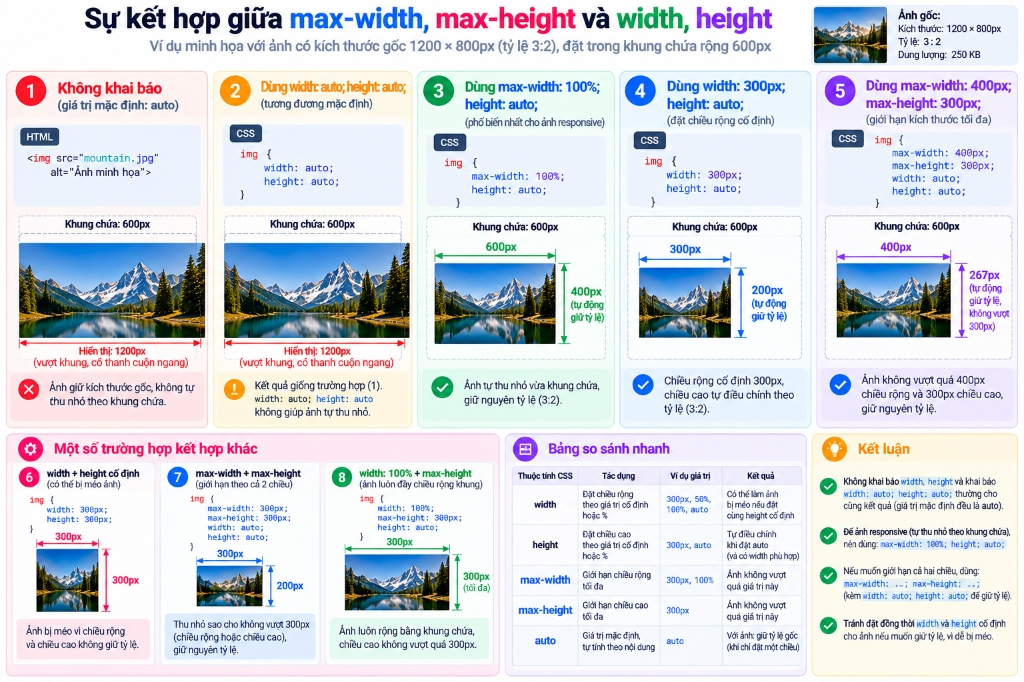
\includegraphics[width=\linewidth]{figures/css_combination_max_dimensions_image.jpg}
\caption{Infographic Toàn Cảnh: Sự Kết Hợp Giữa \codeinline{max-width}, \codeinline{max-height} Và \codeinline{width}, \codeinline{height} Qua 8 Trường Hợp Thực Chiến}
\label{fig:css_combination_max_dimensions_image}
\end{figure}

\begin{enumerate}[leftmargin=1.5em, itemsep=3.5pt, parsep=0pt]
    \item \textbf{Trường hợp 1 (Không khai báo)}: Ảnh lấy kích thước gốc $1200\text{px}$, tràn toang khung chứa $600\text{px}$ và gây thanh cuộn ngang khó chịu.
    \item \textbf{Trường hợp 2 (Dùng \codeinline{width: auto; height: auto;})}: Cho kết quả tương tự Trường hợp 1 (vì \codeinline{auto} trên ảnh là giữ nguyên kích thước pixel gốc của tệp tin).
    \item \textbf{Trường hợp 3 (Dùng \codeinline{max-width: 100\%; height: auto;})}: \term{Chuẩn mực vàng Responsive}: Ảnh tự động thu nhỏ vừa khít chiều rộng khung chứa ($600\text{px}$), chiều cao tự điều chỉnh theo đúng tỷ lệ $3:2$ thành $400\text{px}$.
    \item \textbf{Trường hợp 4 (Dùng \codeinline{width: 300px; height: auto;})}: Chiều rộng bị cố định ở $300\text{px}$, chiều cao tự động tính toán theo tỷ lệ thành $200\text{px}$.
    \item \textbf{Trường hợp 5 (Dùng \codeinline{max-width: 400px; max-height: 300px;} kèm \codeinline{auto})}: Giới hạn kích thước theo cả 2 chiều; ảnh tự động dừng ở $400 \times 267\text{px}$, không vượt quá bất kỳ chiều nào và giữ trọn vẹn tỷ lệ.
    \item \textbf{Trường hợp 6 (Đặt cả \codeinline{width} và \codeinline{height} cố định $300 \times 300\text{px}$)}: \textbf{Lỗi méo ảnh nghiêm trọng}! Tỷ lệ gốc $3:2$ bị bóp méo thành hình vuông $1:1$.
    \item \textbf{Trường hợp 7 (Dùng \codeinline{max-width: 300px; max-height: 300px;} kèm \codeinline{auto})}: Thu nhỏ linh hoạt để không vượt quá $300\text{px}$ ở bất kỳ chiều nào, kết quả đạt $300 \times 200\text{px}$ hoàn hảo.
    \item \textbf{Trường hợp 8 (Dùng \codeinline{width: 100\%; max-height: 300px;})}: Ảnh luôn bung đầy $100\%$ khung chứa ($600\text{px}$), nhưng chiều cao bị chặn đứng ở trần $300\text{px}$.
\end{enumerate}

\begin{prettyTableBox}[Bảng So Sánh Nhanh Tác Dụng Của 4 Thuộc Tính Kích Thước]
\rowcolors{2}{white}{primaryBlue!4}
\begin{tabularx}{\linewidth}{>{\bfseries\color{primaryBlue}}L{2.2cm} Z C{2.2cm} Z}
\rowcolor{primaryBlue}
\thd{Thuộc Tính} & \thd{Tác Dụng Bố Cục} & \thd{Ví Dụ Giá Trị} & \thd{Hành Vi Thực Tế} \\
\codeinline{width} & Đặt chiều rộng cơ sở & \codeinline{300px}, \codeinline{100\%}, \codeinline{auto} & Cố định hoặc co giãn; có thể làm méo ảnh nếu đi cùng height cố định. \\
\codeinline{height} & Đặt chiều cao cơ sở & \codeinline{200px}, \codeinline{auto} & Tự điều chỉnh khi đặt auto (và có width phù hợp). \\
\codeinline{max-width} & Thiết lập trần chiều rộng tối đa & \codeinline{500px}, \codeinline{100\%} & Phần tử không bao giờ nở rộng vượt quá giá trị này. \\
\codeinline{max-height} & Thiết lập trần chiều cao tối đa & \codeinline{300px} & Khóa trần chiều cao, ngăn nội dung kéo dài trang vô tận. \\
\codeinline{auto} & Ủy quyền tính toán cho trình duyệt & \codeinline{auto} & Với ảnh: giữ nguyên tỷ lệ gốc khi chỉ đặt 1 chiều cố định. \\
\end{tabularx}
\end{prettyTableBox}

\begin{noteBox}[Quy Tắc Vàng Khi Kết Hợp max-width / max-height]
\begin{itemize}[leftmargin=1.2em, itemsep=2.5pt, parsep=0pt]
    \item \textbf{Nguyên tắc 1}: Luôn sử dụng \codeinline{max-width} hoặc \codeinline{max-height} khi bạn muốn phần tử \textbf{co giãn mềm dẻo theo nội dung} nhưng không được phép phá vỡ giới hạn khung chứa.
    \item \textbf{Nguyên tắc 2}: \textbf{Tuyệt đối không đặt đồng thời \codeinline{width} và \codeinline{height} cố định} cho các phần tử hình ảnh/video, vì hành động này sẽ phá hủy tỷ lệ khung hình tự nhiên và làm méo mó nội dung.
    \item \textbf{Nguyên tắc 3}: Muốn \codeinline{max-width} hoặc \codeinline{max-height} phát huy toàn bộ sức mạnh responsive, hãy luôn kết hợp chúng với giá trị cơ sở \codeinline{width: auto;} hoặc \codeinline{height: auto;}.
\end{itemize}
\end{noteBox}

% ------------------------------------------------------------------------------
% 3.4 ẢNH HƯỞNG TỪ DISPLAY VÀ POSITION
% ------------------------------------------------------------------------------
\subsection{Mối Tương Quan \& Ảnh Hưởng Từ \csshint{display} Và \csshint{position}}
\label{subsec:display_position_impact}

Hành vi của \codeinline{width} và \codeinline{height} phụ thuộc mật thiết vào cách phần tử được định kiểu hiển thị (\term{display mode}) và định vị (\term{positioning context}).

\begin{browserWindow}[Mô Phỏng Trực Quan 3 Chế Độ Hiển Thị \& Định Vị]
\centering
\begin{tikzpicture}[scale=0.96, every node/.style={transform shape}]
  % KHỐI 1: display: inline
  \begin{scope}[shift={(0, 0)}]
    \draw[fill=gray!4, draw=gray!25, rounded corners=6pt] (-2.25, -2.25) rectangle (2.25, 2.05);
    \node[anchor=north, font=\small\bfseries\color{accentOrange!90!black}] at (0, 1.85) {1. display: inline;};
    \node[anchor=north, font=\fontsize{7.5pt}{9pt}\selectfont\color{gray!70}] at (0, 1.35) {Thẻ nội dòng (span, a, em)};
    
    \draw[fill=white, draw=gray!25, rounded corners=4pt] (-1.95, -1.4) rectangle (1.95, 0.8);
    \node[anchor=north west, font=\fontsize{7.5pt}{9pt}\selectfont\color{darkText!75}] at (-1.8, 0.65) {Dòng văn bản:};
    
    % Thẻ inline thực tế
    \draw[fill=accentOrange!15, draw=accentOrange, line width=1pt, rounded corners=3pt] (-1.8, -0.25) rectangle (-0.45, 0.3);
    \node[anchor=center, font=\fontsize{7pt}{8.5pt}\selectfont\bfseries\color{accentOrange!90!black}] at (-1.125, 0.025) {inline text};
    \node[anchor=west, font=\fontsize{7pt}{8.5pt}\selectfont\color{darkText!50}] at (-0.35, 0.025) {văn bản...};
    
    % Khung bị lờ đi
    \draw[dashed, draw=dangerRed!90!black, line width=0.9pt] (-1.8, -0.8) rectangle (0.6, 0.3);
    \node[anchor=north, font=\fontsize{6.5pt}{7.5pt}\selectfont\bfseries\color{dangerRed!90!black}] at (-0.6, -0.82) {Khung 90x32px bị lờ đi!};
    
    \node[anchor=center, font=\fontsize{7pt}{8.5pt}\selectfont\bfseries\color{dangerRed}, fill=dangerRed!10, draw=dangerRed!30, rounded corners=3pt, inner sep=3pt] at (0, -1.82) {[BỊ LỜ ĐI] Không nhận size};
  \end{scope}

  % KHỐI 2: display: inline-block
  \begin{scope}[shift={(4.9, 0)}]
    \draw[fill=gray!4, draw=gray!25, rounded corners=6pt] (-2.25, -2.25) rectangle (2.25, 2.05);
    \node[anchor=north, font=\small\bfseries\color{successGreen!85!black}] at (0, 1.85) {2. display: inline-block;};
    \node[anchor=north, font=\fontsize{7.5pt}{9pt}\selectfont\color{gray!70}] at (0, 1.35) {Khối lai đứng cùng dòng};
    
    \draw[fill=white, draw=gray!25, rounded corners=4pt] (-1.95, -1.4) rectangle (1.95, 0.8);
    \node[anchor=north west, font=\fontsize{7.5pt}{9pt}\selectfont\color{darkText!75}] at (-1.8, 0.65) {Dòng văn bản:};
    
    \draw[fill=successGreen!15, draw=successGreen!90!black, line width=1.1pt, rounded corners=3pt] (-1.8, -0.6) rectangle (0.6, 0.3);
    \node[anchor=center, font=\fontsize{6.8pt}{8pt}\selectfont\bfseries\color{successGreen!85!black}] at (-0.6, -0.15) {inline-block (90x32px)};
    \node[anchor=west, font=\fontsize{7pt}{8.5pt}\selectfont\color{darkText!50}] at (0.75, -0.15) {văn bản...};
    
    \draw[{Stealth[length=3pt]}-{Stealth[length=3pt]}, successGreen!85!black, line width=0.6pt] (-1.8, -0.9) -- (0.6, -0.9);
    \node[anchor=north, font=\fontsize{6.5pt}{7.5pt}\selectfont\bfseries\color{successGreen!85!black}] at (-0.6, -0.92) {Rộng thực tế: đúng 90px};
    
    \node[anchor=center, font=\fontsize{7pt}{8.5pt}\selectfont\bfseries\color{successGreen!85!black}, fill=successGreen!12, draw=successGreen!35, rounded corners=3pt, inner sep=3pt] at (0, -1.82) {[CHUẨN] Nhận size đầy đủ};
  \end{scope}

  % KHỐI 3: position: absolute
  \begin{scope}[shift={(9.8, 0)}]
    \draw[fill=gray!4, draw=gray!25, rounded corners=6pt] (-2.25, -2.25) rectangle (2.25, 2.05);
    \node[anchor=north, font=\small\bfseries\color{primaryBlue}] at (0, 1.85) {3. position: absolute;};
    \node[anchor=north, font=\fontsize{7.5pt}{9pt}\selectfont\color{gray!70}] at (0, 1.35) {Tách khỏi normal flow};
    
    \draw[fill=white, draw=gray!25, rounded corners=4pt] (-1.95, -1.4) rectangle (1.95, 0.8);
    
    \draw[fill=slateBg!70, draw=gray!40, dashed, line width=0.8pt, rounded corners=3pt] (-1.8, -1.2) rectangle (1.8, 0.65);
    \node[anchor=north west, font=\fontsize{6.5pt}{7.5pt}\selectfont\color{gray!60}] at (-1.7, 0.6) {Parent (.relative)};
    
    \draw[fill=primaryBlue!20, draw=primaryBlue, line width=1.1pt, rounded corners=2pt] (-1.8, -1.2) rectangle (1.8, 0.15);
    \node[anchor=center, font=\fontsize{7pt}{8.5pt}\selectfont\bfseries\color{primaryBlue}] at (0, -0.3) {Overlay (100\% $\times$ 100\%)};
    \node[anchor=north, font=\fontsize{5.8pt}{7pt}\selectfont\color{primaryBlue!85!black}] at (0, -0.58) {top:0; bottom:0; left:0; right:0;};
    
    \node[anchor=center, font=\fontsize{7pt}{8.5pt}\selectfont\bfseries\color{primaryBlue}, fill=primaryBlue!12, draw=primaryBlue!35, rounded corners=3pt, inner sep=3pt] at (0, -1.82) {[TÁCH LUỒNG] Tự do phủ kín};
  \end{scope}
\end{tikzpicture}
\end{browserWindow}

\vspace{2pt}

\begin{tcolorbox}[
    enhanced,
    colback=white,
    colframe=accentOrange!70!black,
    arc=4pt,
    boxrule=0.8pt,
    leftrule=3.5pt,
    top=4pt, bottom=4pt, left=8pt, right=8pt,
    before=\par\vspace{3pt}\noindent,
    after=\par\vspace{3pt}
]
{\bfseries\color{accentOrange!90!black}\normalsize 1. Chế độ hiển thị nội dòng (\codeinline{display: inline;}):}
\begin{itemize}[leftmargin=1.2em, itemsep=2pt, parsep=0pt, topsep=2pt]
    \item Các phần tử nội dòng (như \codeinline{<a>}, \codeinline{<span>}, \codeinline{<strong>}, \codeinline{<em>}) sẽ \textbf{hoàn toàn không nhận} các thuộc tính \codeinline{width}, \codeinline{height}, \codeinline{margin-top}, \codeinline{margin-bottom}, \codeinline{padding-top}, và \codeinline{padding-bottom} theo cách thông thường.
    \item Chiều rộng và chiều cao của chúng được xác định hoàn toàn bởi dung lượng chữ bên trong.
\end{itemize}
\end{tcolorbox}

\begin{tcolorbox}[
    enhanced,
    colback=white,
    colframe=successGreen!75!black,
    arc=4pt,
    boxrule=0.8pt,
    leftrule=3.5pt,
    top=4pt, bottom=4pt, left=8pt, right=8pt,
    before=\par\vspace{3pt}\noindent,
    after=\par\vspace{3pt}
]
{\bfseries\color{successGreen!85!black}\normalsize 2. Chế độ khối nội dòng (\codeinline{display: inline-block;}):}
\begin{itemize}[leftmargin=1.2em, itemsep=2pt, parsep=0pt, topsep=2pt]
    \item Các phần tử này thừa hưởng khả năng thiết lập \codeinline{width} và \codeinline{height} độc lập như một khối (\term{block}), nhưng đồng thời vẫn nằm thẳng hàng trên cùng một dòng với các phần tử nội dòng khác.
\end{itemize}
\end{tcolorbox}

\begin{tcolorbox}[
    enhanced,
    colback=white,
    colframe=primaryBlue,
    arc=4pt,
    boxrule=0.8pt,
    leftrule=3.5pt,
    top=4pt, bottom=4pt, left=8pt, right=8pt,
    before=\par\vspace{3pt}\noindent,
    after=\par\vspace{3pt}
]
{\bfseries\color{primaryBlue}\normalsize 3. Chế độ định vị thoát luồng (\codeinline{position: absolute;} / \codeinline{position: fixed;}):}
\begin{itemize}[leftmargin=1.2em, itemsep=2pt, parsep=0pt, topsep=2pt]
    \item Khi một phần tử được định vị tuyệt đối hoặc cố định, nó sẽ \textbf{bị rút hoàn toàn khỏi dòng chảy tài liệu thông thường} (\term{normal document flow}).
    \item \codeinline{width} và \codeinline{height} của chúng có thể được thiết lập độc lập hoặc có thể dùng đồng thời cặp thuộc tính vị trí \codeinline{top: 0; bottom: 0;} và \codeinline{left: 0; right: 0;} để tự động kéo giãn phủ kín không gian.
    \item \textbf{Ví dụ điển hình}: Khai báo \codeinline{width: 100\%; height: 100\%; position: absolute; top: 0; left: 0;} sẽ làm cho lớp phủ (\term{overlay}) lấp đầy toàn bộ phần tử cha gần nhất có khai báo \codeinline{position} khác \codeinline{static}.
\end{itemize}
\end{tcolorbox}

\clearpage

% ------------------------------------------------------------------------------
% 3.5 TƯƠNG TÁC GIỮA OVERFLOW VÀ KÍCH THƯỚC CỐ ĐỊNH
% ------------------------------------------------------------------------------
\subsection{Tương Tác Giữa \csshint{overflow} Và Kích Thước \csshint{width} / \csshint{height}}
\label{subsec:overflow_interaction}

Khi bạn thiết lập \codeinline{width} hoặc \codeinline{height} cố định cho một phần tử và khối lượng nội dung bên trong lại lớn hơn không gian kích thước đó, thuộc tính \codeinline{overflow} sẽ quyết định cách thức trình duyệt xử lý phần nội dung bị tràn:

\begin{figure}[H]
\centering
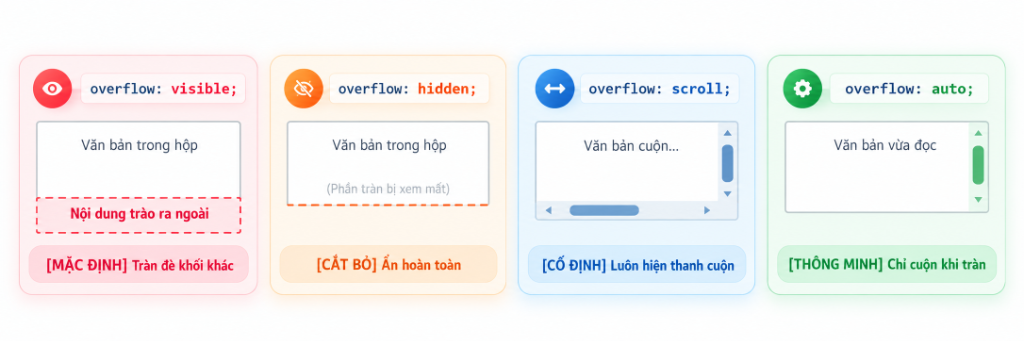
\includegraphics[width=\linewidth]{figures/css_overflow_four_modes_cards.png}
\caption{Mô Phỏng Trực Quan 4 Cơ Chế Xử Lý Của Thuộc Tính \codeinline{overflow} (visible, hidden, scroll, auto)}
\label{fig:css_overflow_four_modes}
\end{figure}

\begin{itemize}[leftmargin=1.5em, itemsep=4pt, parsep=0pt]
    \item \textbf{\codeinline{overflow: visible;}} (\textbf{Mặc định}): Nội dung bị tràn sẽ không bị cắt bỏ mà tràn ra ngoài đường biên của phần tử, đè lên các khối giao diện khác ở phía dưới.
    \item \textbf{\codeinline{overflow: hidden;}}: Phần nội dung bị tràn ra ngoài kích thước hộp sẽ bị cắt bỏ thẳng tay và hoàn toàn ẩn đi, người dùng không thể xem được.
    \item \textbf{\codeinline{overflow: scroll;}}: Luôn luôn hiển thị thanh cuộn (dù nội dung có bị tràn hay không), cho phép người dùng cuộn xem toàn bộ dữ liệu.
    \item \textbf{\codeinline{overflow: auto;}}: Trình duyệt thông minh chỉ hiển thị thanh cuộn khi nội dung thực sự bị tràn vượt quá giới hạn của hộp chứa.
\end{itemize}

% ------------------------------------------------------------------------------
% 3.6 LỜI KHUYÊN QUAN TRỌNG VÀ RESET TOÀN CỤC CHUẨN
% ------------------------------------------------------------------------------
\subsection{Lời Khuyên Quan Trọng \& Thiết Lập Reset Toàn Cục Chuẩn}
\label{subsec:global_box_sizing_recommendation}

\begin{tipBox}[Quy Tắc Vàng Khởi Đầu Cho Mọi Dự Án Web Hiện Đại]
Trong hầu hết mọi dự án web hiện đại (từ website cá nhân cho tới các ứng dụng doanh nghiệp quy mô lớn), bạn nên \textbf{luôn luôn bắt đầu bằng việc thiết lập \codeinline{box-sizing: border-box;} cho tất cả các phần tử} trong tệp tin CSS reset hoặc stylesheet toàn cục:

\begin{lstlisting}[language=CSS3]
*, *::before, *::after {
    box-sizing: border-box;
}
\end{lstlisting}

\textbf{Lợi ích thực tế}: Thiết lập này sẽ giúp bạn quản lý kích thước các phần tử một cách trực quan và dễ dàng hơn rất nhiều. Mọi con số \codeinline{width} và \codeinline{height} bạn đặt ra sẽ luôn đúng tuyệt đối với diện tích chiếm chỗ trên màn hình, loại bỏ vĩnh viễn những lỗi tính toán sai lệch kích thước gây vỡ bố cục khi thêm \codeinline{padding} và \codeinline{border}.
\end{tipBox}

% ==============================================================================
% MỤC 4: CHUYÊN ĐỀ THỰC CHIẾN: LÀM CHỦ THUỘC TÍNH MAX-WIDTH
% ==============================================================================
\clearpage
\section{Chuyên Đề Thực Chiến: Làm Chủ Thuộc Tính \csshint{max-width} (Responsive Masterclass)}
\label{sec:max_width_masterclass}

Trong thiết kế web hiện đại, \term{Responsive Web Design} (thiết kế thích ứng đa thiết bị) là tiêu chuẩn bắt buộc. Nếu như \codeinline{width} đại diện cho sự áp đặt kích thước cố định, thì \codeinline{max-width} chính là chìa khóa mở ra sự linh hoạt và giải phóng trang web khỏi nguy cơ vỡ khung bố cục trên các màn hình nhỏ.

% ------------------------------------------------------------------------------
% 4.1 KHÁI NIỆM & Ý NGHĨA
% ------------------------------------------------------------------------------
\subsection{Khái Niệm \& Ý Nghĩa Cốt Lõi Của \csshint{max-width}}
\label{subsec:max_width_concept}

Thuộc tính \codeinline{max-width} dùng để \textbf{giới hạn chiều rộng tối đa} mà một phần tử HTML có thể đạt tới. Nếu nội dung hoặc kích thước màn hình hiển thị nhỏ hơn giá trị \codeinline{max-width}, phần tử sẽ tự động co lại để vừa khít với không gian có sẵn.

\begin{codeWindow}[Cú Pháp Thiết Lập max-width Cơ Bản]
\begin{lstlisting}[language=CSS3]
.element {
    max-width: 500px;
}
\end{lstlisting}
\end{codeWindow}

\begin{conceptBox}[Cơ Chế Hoạt Động 2 Trạng Thái Của max-width]
Khi thiết lập \codeinline{max-width: 500px;}, trình duyệt sẽ tuân thủ nghiêm ngặt 2 nguyên tắc sau:
\begin{enumerate}[leftmargin=1.5em, itemsep=3pt, parsep=0pt]
    \item \textbf{Nếu phần tử rộng hơn $500\text{px}$}: Nó sẽ bị chặn lại ở ngưỡng trần tối đa đúng bằng $500\text{px}$, không bao giờ vượt qua.
    \item \textbf{Nếu phần tử nhỏ hơn $500\text{px}$}: Nó vẫn giữ nguyên kích thước tự nhiên của mình mà không bị ép buộc phải phình to ra $500\text{px}$.
\end{enumerate}
\end{conceptBox}

\subsubsection{Ý Nghĩa Then Chốt Trong Thiết Kế UI/UX}
\begin{itemize}[leftmargin=1.5em, itemsep=3pt, parsep=0pt]
    \item \textbf{Giới hạn chiều rộng tối đa của phần tử}: Giữ cho các khối nội dung không bị bè quá rộng trên màn hình Desktop lớn hoặc màn hình Ultra-Wide, duy trì độ dài dòng đọc lý tưởng theo công thái học thị giác.
    \item \textbf{Tăng cường tính linh hoạt}: Giúp giao diện hiển thị xuất sắc, mượt mà trên mọi kích cỡ màn hình từ điện thoại bỏ túi, máy tính bảng cho đến màn hình tivi lớn.
    \item \textbf{Bộ đôi hoàn hảo với \codeinline{width: 100\%}}: Đây là công thức phối hợp kinh điển nhất trong kỹ nghệ dựng layout responsive hiện đại.
\end{itemize}

\begin{figure}[H]
\centering
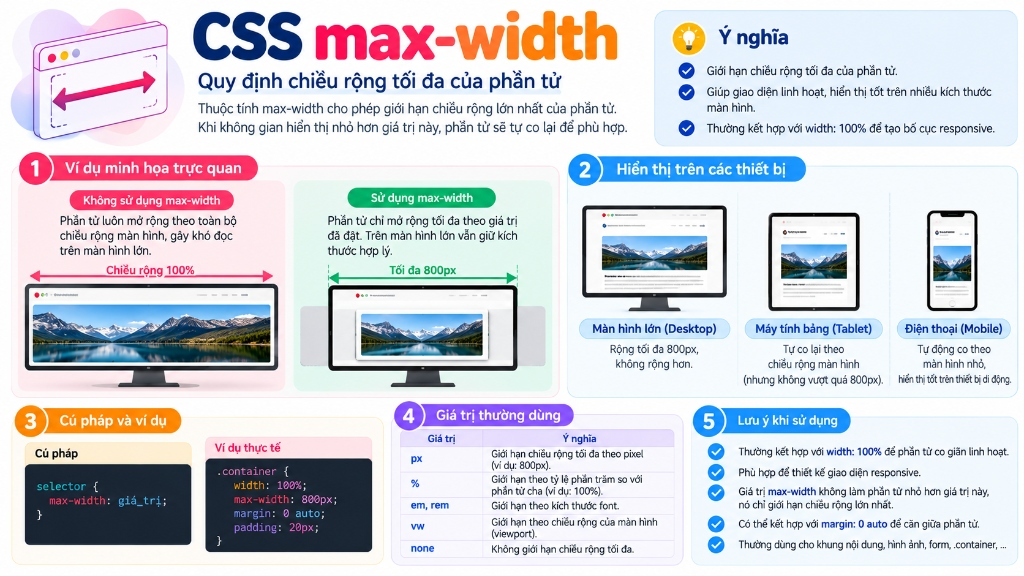
\includegraphics[width=0.98\linewidth]{figures/max_width_infographic_overview.jpg}
\caption{Infographic Toàn Diện: Khái Niệm, Cơ Chế Hiển Thị Đa Thiết Bị \& Cú Pháp max-width}
\label{fig:max_width_infographic_overview}
\end{figure}

% ------------------------------------------------------------------------------
% 4.2 SỰ KHÁC BIỆT GIỮA WIDTH VÀ MAX-WIDTH
% ------------------------------------------------------------------------------
\subsection{Sự Khác Biệt Giữa \csshint{width} Và \csshint{max-width}}
\label{subsec:diff_width_vs_max_width}

Sự nhầm lẫn giữa \codeinline{width} và \codeinline{max-width} là một trong những nguyên nhân hàng đầu gây ra lỗi thanh cuộn ngang (\term{Horizontal Scrollbar}) trên các thiết bị di động.

\begin{prettyTableBox}[Bảng So Sánh Cơ Chế Hoạt Động: width: 500px vs max-width: 500px]
\rowcolors{2}{white}{primaryBlue!4}
\sffamily\small
\begin{tabularx}{\linewidth}{|>{\raggedright\arraybackslash \ttfamily\color{primaryBlue}\bfseries}K{3.4cm}|Z|}
\hline
\rowcolor{primaryBlue} \thd{\sffamily Thuộc tính} & \thd{\sffamily Cách thức hoạt động của trình duyệt} \\
\hline
width: 500px; & Phần tử \textbf{luôn luôn bị khóa cứng} ở chiều rộng đúng $500\text{px}$ bất kể kích thước màn hình thiết bị hay phần tử cha lớn hay nhỏ. \\
\hline
max-width: 500px; & Phần tử \textbf{có thể nhỏ hơn $500\text{px}$} khi không gian bị thu hẹp, nhưng \textbf{tuyệt đối không bao giờ lớn hơn $500\text{px}$}. \\
\hline
\end{tabularx}
\end{prettyTableBox}

\subsubsection{Ví Dụ Mã Nguồn So Sánh Trực Tiếp}

\begin{codeWindow}[Ví Dụ So Sánh Hai Khối: .box1 (width) vs .box2 (max-width)]
\begin{lstlisting}[language=CSS3, escapeinside={(*@}{@*)}]
/* Khoi 1: Dung width co dinh */
.box1 {
    width: 500px;
    background: #e53935; /* Do */
    color: white;
    padding: 12px;
}

/* Khoi 2: Dung max-width linh hoat */
.box2 {
    max-width: 500px;
    background: #1e88e5; /* Xanh duong */
    color: white;
    padding: 12px;
}
\end{lstlisting}
\end{codeWindow}

\begin{warnBox}[Hành Vi Hiển Thị Khi Cửa Sổ Trình Duyệt Nhỏ Hơn 500px (Ví dụ Mobile 375px)]
\begin{itemize}[leftmargin=1.5em, itemsep=3pt, parsep=0pt]
    \item \textbf{Đối với \codeinline{.box1} (\codeinline{width: 500px;})}: Phần tử \textbf{vẫn giữ nguyên $500\text{px}$}, vượt quá kích thước $375\text{px}$ của màn hình. Kết quả: \textbf{Xuất hiện thanh cuộn ngang}, nội dung bị tràn ra ngoài rìa màn hình, gây vỡ hoàn toàn layout website!
    \item \textbf{Đối với \codeinline{.box2} (\codeinline{max-width: 500px;})}: Phần tử \textbf{tự động co lại bằng đúng $375\text{px}$} để vừa vặn hoàn hảo với màn hình điện thoại. Giao diện mượt mà, không sinh thanh cuộn ngang, bố cục được bảo toàn nguyên vẹn.
\end{itemize}
\end{warnBox}

\begin{figure}[H]
\centering
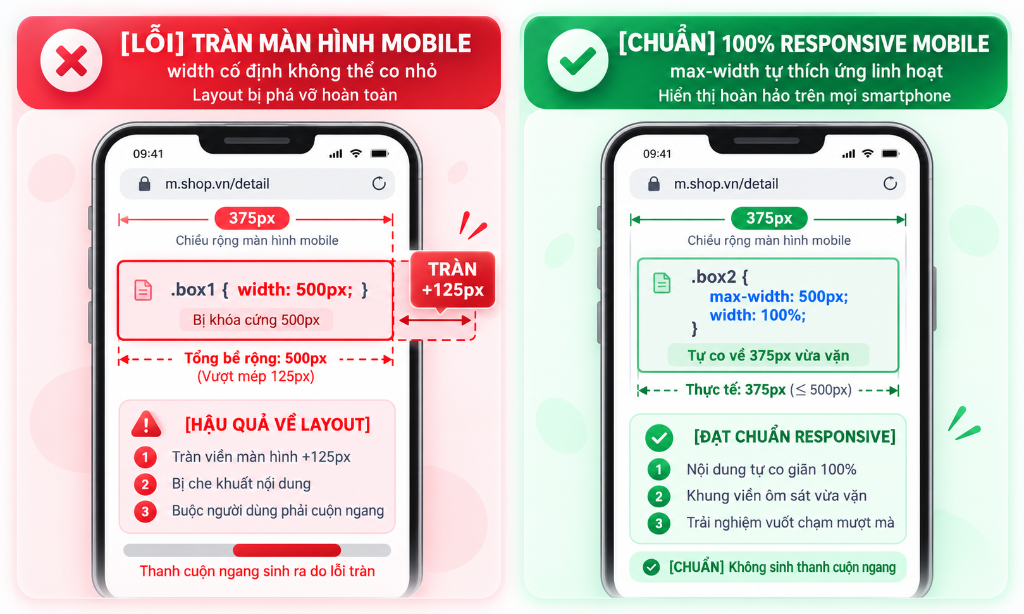
\includegraphics[width=0.96\linewidth]{figures/width_vs_max_width_mobile_comparison.png}
\caption{Đối Chiếu Trực Quan Trên Thiết Bị Di Động: \codeinline{width: 500px} (Gây Tràn 125px) vs \codeinline{max-width: 500px} (Tự Co Giãn Vừa Vặn)}
\label{fig:width_vs_max_width_mobile_comparison}
\end{figure}

% ------------------------------------------------------------------------------
% 4.3 CÁC VÍ DỤ ỨNG DỤNG THỰC TẾ
% ------------------------------------------------------------------------------
\subsection{Các Ví Dụ Ứng Dụng Thực Tế Của \csshint{max-width}}
\label{subsec:practical_max_width_applications}

\subsubsection{Ứng Dụng 1: Giới Hạn Chiều Rộng Tối Đa Cho Hình Ảnh (Responsive Images)}

Đây là đoạn mã quan trọng hàng đầu trong mọi stylesheet CSS hiện đại để bảo đảm hình ảnh hiển thị hoàn hảo:

\begin{codeWindow}[Quy Tắc Hình Ảnh Đáp Ứng Chuẩn Công Nghiệp]
\begin{lstlisting}[language=CSS3]
img {
    max-width: 100%;
    height: auto;
    display: block;
}
\end{lstlisting}
\end{codeWindow}

\begin{conceptBox}[Tác Dụng Kỹ Thuật]
\begin{itemize}[leftmargin=1.5em, itemsep=3pt, parsep=0pt]
    \item \textbf{Không bao giờ vượt quá kích thước gốc}: Bức ảnh giữ nguyên độ nét, không bị kéo vỡ hạt (\term{pixelated}) khi container quá lớn.
    \item \textbf{Tự động co nhỏ}: Khi kích thước màn hình nhỏ hơn chiều rộng thực của ảnh, \codeinline{max-width: 100\%;} ép ảnh co nhỏ lại đúng bằng chiều rộng phần tử cha.
    \item \textbf{\codeinline{height: auto;}}: Đảm bảo tỷ lệ khung hình (\term{aspect ratio}) luôn được khóa chuẩn, ảnh không bao giờ bị méo mó hình học.
\end{itemize}
\end{conceptBox}

\begin{figure}[H]
\centering
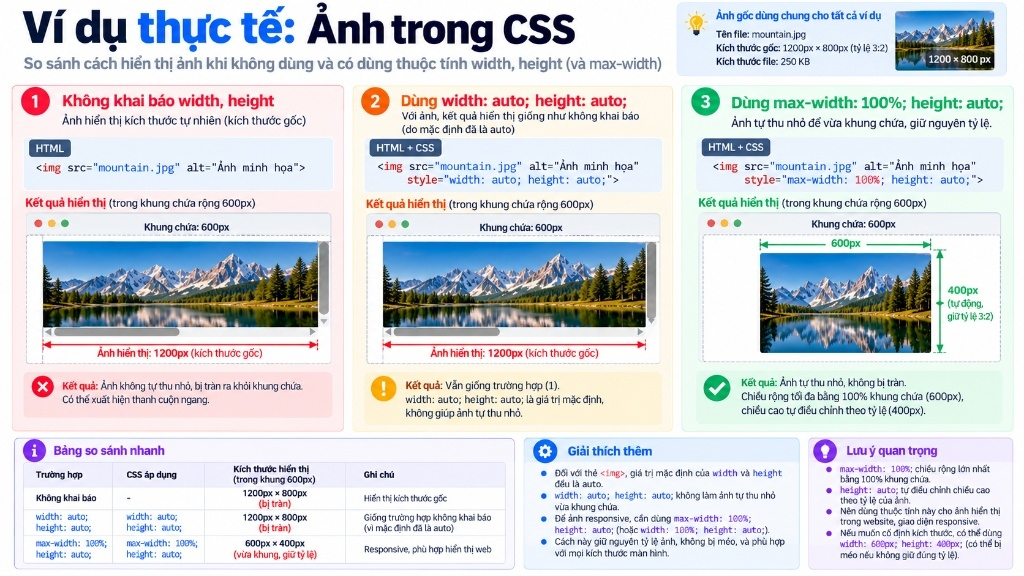
\includegraphics[width=\linewidth]{figures/css_image_auto_vs_max_width_comparison.jpg}
\caption{Ví Dụ Thực Tế Ảnh Trong CSS: So Sánh 3 Trường Hợp (Không Khai Báo, Dùng auto Và Dùng max-width: 100\%; height: auto;)}
\label{fig:css_image_auto_vs_max_width_comparison}
\end{figure}

\subsubsection{Ứng Dụng 2: Tạo Khung Chứa Nội Dung Trung Tâm (Responsive Container)}

Trong thiết kế giao diện website, các lập trình viên thường dùng lớp \codeinline{.container} để bao bọc toàn bộ nội dung của trang:

\begin{codeWindow}[Mẫu Responsive Container Kinh Điển]
\begin{lstlisting}[language=CSS3]
.container {
    max-width: 1200px;
    width: 90%;
    margin: 0 auto;
}
\end{lstlisting}
\end{codeWindow}

\begin{prettyTableBox}[Cơ Chế Thích Ứng Của Lớp .container Trên Các Môi Trường Màn Hình]
\rowcolors{2}{white}{primaryBlue!4}
\sffamily\small
\begin{tabularx}{\linewidth}{|>{\raggedright\arraybackslash \sffamily\bfseries\color{primaryBlue}}K{3.8cm}|Z|}
\hline
\rowcolor{primaryBlue} \thd{\sffamily Môi trường hiển thị} & \thd{\sffamily Hành vi hiển thị thực tế của .container} \\
\hline
Màn hình lớn (Desktop / 4K \newline Width $> 1333\text{px}$) & \codeinline{max-width: 1200px;} kích hoạt. Trang web được giữ cố định ở bề rộng tối đa $1200\text{px}$, căn giữa màn hình nhờ \codeinline{margin: 0 auto;}, không bị kéo dãn quá đà. \\
\hline
Màn hình nhỏ hơn \newline (Laptop / Tablet / Mobile) & \codeinline{width: 90\%;} chiếm ưu thế. Khung chứa tự động chiếm trọn $90\%$ chiều rộng màn hình, để lại $5\%$ khoảng đệm ở mỗi bên lề trái/phải cực kỳ thanh lịch. \\
\hline
\end{tabularx}
\end{prettyTableBox}

\begin{figure}[H]
\centering
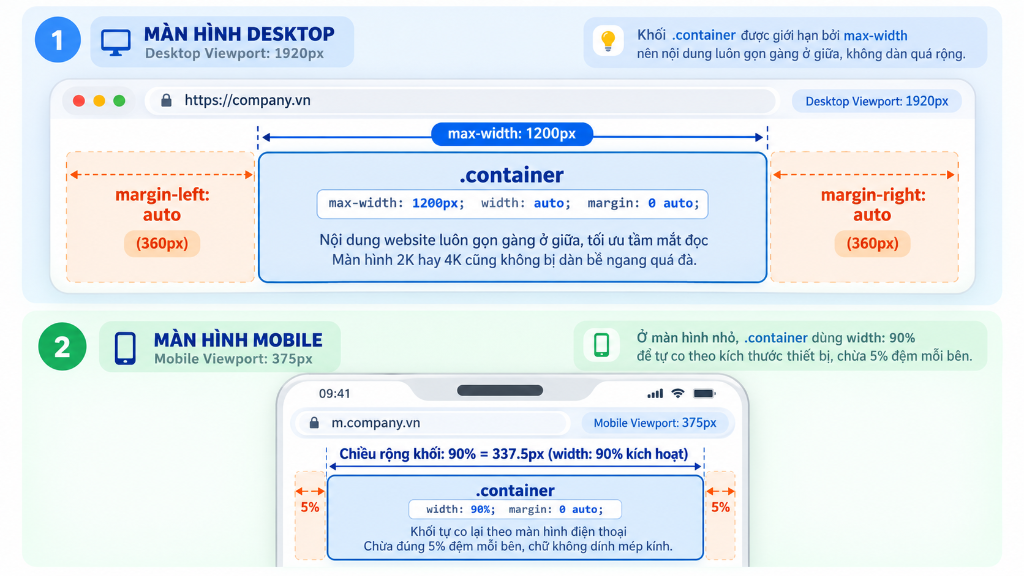
\includegraphics[width=\linewidth]{figures/max_width_container_desktop_mobile.png}
\caption{Mô Phỏng Thực Tế Lớp \codeinline{.container}: Cố Định 1200px Trên Desktop \& Co Giãn 90\% Trên Mobile}
\label{fig:max_width_container_desktop_mobile}
\end{figure}

\subsubsection{Ứng Dụng 3: Khung Đọc Văn Bản Công Thái Học (Blog \& Báo Điện Tử)}

\begin{codeWindow}[Khung Chứa Nội Dung Đọc Tiêu Chuẩn 800px]
\begin{lstlisting}[language=CSS3]
.article-container {
    width: 100%;
    max-width: 800px;
    margin: 0 auto;
    padding: 20px;
}
\end{lstlisting}
\end{codeWindow}

% ------------------------------------------------------------------------------
% 4.4 KẾT HỢP MAX-WIDTH VÀ MIN-WIDTH
% ------------------------------------------------------------------------------
\subsection{4. Kỹ Thuật Phối Hợp: \csshint{max-width} Kết Hợp Với \csshint{min-width}}
\label{subsec:combine_min_max_width}

Khi cần kiểm soát kích thước trong một dải biên độ an toàn tuyệt đối, việc kết hợp đồng thời \codeinline{min-width} và \codeinline{max-width} là kỹ thuật tối thượng.

\begin{prettyTableBox}[Ý Nghĩa Cặp Thuộc Tính Giới Hạn Biên Độ]
\rowcolors{2}{white}{primaryBlue!4}
\sffamily\small
\begin{tabularx}{\linewidth}{|>{\raggedright\arraybackslash \ttfamily\color{primaryBlue}\bfseries}K{3.4cm}|Z|}
\hline
\rowcolor{primaryBlue} \thd{\sffamily Thuộc tính} & \thd{\sffamily Ý nghĩa \& Ngưỡng giới hạn} \\
\hline
max-width & Giới hạn \textbf{ngưỡng trần tối đa} của phần tử (không thể to hơn). \\
\hline
min-width & Giới hạn \textbf{ngưỡng sàn tối thiểu} của phần tử (không thể nhỏ hơn). \\
\hline
\end{tabularx}
\end{prettyTableBox}

\begin{codeWindow}[Ví Dụ Phối Hợp 3 Cấp Độ Kích Thước Hoàn Hảo]
\begin{lstlisting}[language=CSS3]
.box {
    min-width: 300px;
    max-width: 600px;
    width: 80%;
}
\end{lstlisting}
\end{codeWindow}

\begin{conceptBox}[Cơ Chế Phân Bổ Kích Thước 3 Kịch Bản Theo Độ Rộng Màn Hình ($W$)]
\begin{enumerate}[leftmargin=1.5em, itemsep=3pt, parsep=0pt]
    \item \textbf{Khi màn hình rất hẹp ($W < 375\text{px}$)}: $80\% \times W < 300\text{px}$, thuộc tính \codeinline{min-width: 300px;} sẽ can thiệp để giữ kích thước tối thiểu là $300\text{px}$, bảo đảm các nút bấm hay văn bản bên trong không bị dồn nén đến mức mất chữ.
    \item \textbf{Khi màn hình nằm trong khoảng lý tưởng ($375\text{px} \le W \le 750\text{px}$)}: Khối co giãn mượt mà đúng bằng $80\%$ độ rộng màn hình ($80\% \times W$), tạo cảm giác thoáng đãng và tự nhiên.
    \item \textbf{Khi màn hình rất rộng ($W > 750\text{px}$)}: $80\% \times W > 600\text{px}$, thuộc tính \codeinline{max-width: 600px;} sẽ chặn đứng kích thước tại ngưỡng $600\text{px}$, ngăn chặn phần tử bị phình to bất thường.
\end{enumerate}
\end{conceptBox}

\begin{figure}[H]
\centering
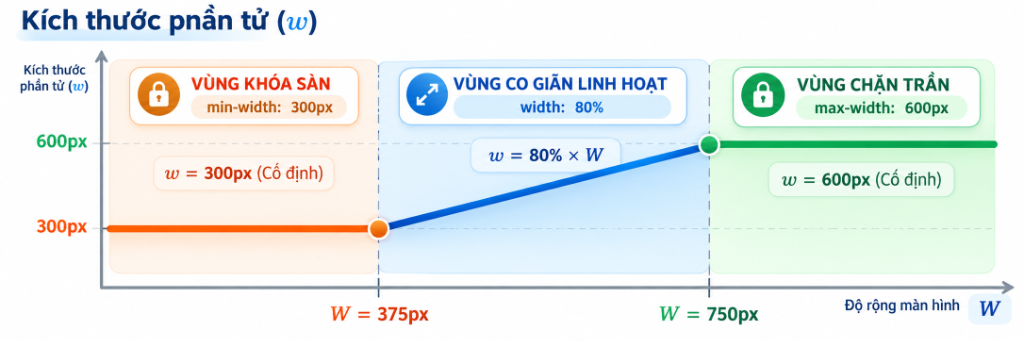
\includegraphics[width=\linewidth]{figures/clamp_min_max_width_graph.png}
\caption{Đồ Thị Trực Quan: Cơ Chế Clamping Ba Cấp Độ Kết Hợp \codeinline{min-width}, \codeinline{width} Và \codeinline{max-width}}
\label{fig:clamp_min_max_width_graph}
\end{figure}

% ------------------------------------------------------------------------------
% 4.5 THỰC NGHIỆM THỰC TẾ VỚI LỚP .MAX VÀ DEVTOOLS
% ------------------------------------------------------------------------------
\subsection{Thực Nghiệm Thực Tế Với Lớp \csshint{.MAX} \& Đối Chiếu Chrome DevTools}
\label{subsec:experiment_class_max}

Để kiểm chứng bản chất tính toán của trình duyệt, chúng ta cùng phân tích một thực nghiệm cụ thể với lớp CSS \codeinline{.MAX}:

\begin{codeWindow}[Mã Nguồn Thực Nghiệm Lớp .MAX]
\begin{lstlisting}[language=CSS3]
.MAX {
    background: red;
    max-width: 500px;
    height: 300px;
    font-size: 20px;
}
\end{lstlisting}
\end{codeWindow}

\subsubsection{Phân Tích Cách Hoạt Động Cốt Lõi}
\begin{enumerate}[leftmargin=1.5em, itemsep=3pt, parsep=0pt]
    \item \textbf{\codeinline{max-width: 500px;}}: Phần tử có chiều rộng tối đa là $500\text{px}$. Nếu trình duyệt nhỏ hơn $500\text{px}$, phần tử co lại theo kích thước của nó; nếu trình duyệt lớn hơn $500\text{px}$, phần tử không vượt quá $500\text{px}$.
    \item \textbf{\codeinline{height: 300px;}}: Chiều cao của phần tử luôn là $300\text{px}$, không thay đổi dù viewport rộng hay hẹp.
    \item \textbf{\codeinline{font-size: 20px;}}: Cỡ chữ của nội dung văn bản bên trong được thiết lập cố định $20\text{px}$.
\end{enumerate}

\subsubsection{Điều Gì Sẽ Xảy Ra Khi Viewport Nhỏ Hơn 500px?}
\begin{itemize}[leftmargin=1.5em, itemsep=3pt, parsep=0pt]
    \item \textbf{Nếu màn hình thu hẹp còn khoảng $400\text{px}$}: Khối \codeinline{.MAX} sẽ tự động co lại bằng khoảng $400\text{px}$ (cụ thể trên thực nghiệm Chrome DevTools đo được chính xác là $\mathbf{398.4\text{px} \times 300\text{px}}$ do trừ viền mép cửa sổ).
    \item \textbf{Nếu màn hình mở rộng ra $600\text{px}$ hoặc hơn}: Khối \codeinline{.MAX} vẫn chỉ rộng đúng $\mathbf{500\text{px} \times 300\text{px}}$, không hề tăng thêm.
\end{itemize}

\begin{figure}[H]
\centering
\begin{subfigure}[b]{0.48\linewidth}
    \centering
    \setlength{\fboxsep}{0pt}\setlength{\fboxrule}{0.8pt}
    \fcolorbox{gray!30}{white}{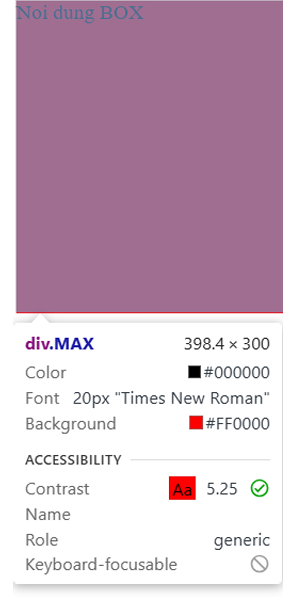
\includegraphics[height=6.2cm, keepaspectratio]{figures/max_width_devtools_narrow_398px_clean.png}}
    \caption{Viewport hẹp ($< 500\text{px}$): Co về $398.4\text{px} \times 300\text{px}$}
    \label{subfig:devtools_narrow}
\end{subfigure}
\hfill
\begin{subfigure}[b]{0.48\linewidth}
    \centering
    \setlength{\fboxsep}{0pt}\setlength{\fboxrule}{0.8pt}
    \fcolorbox{gray!30}{white}{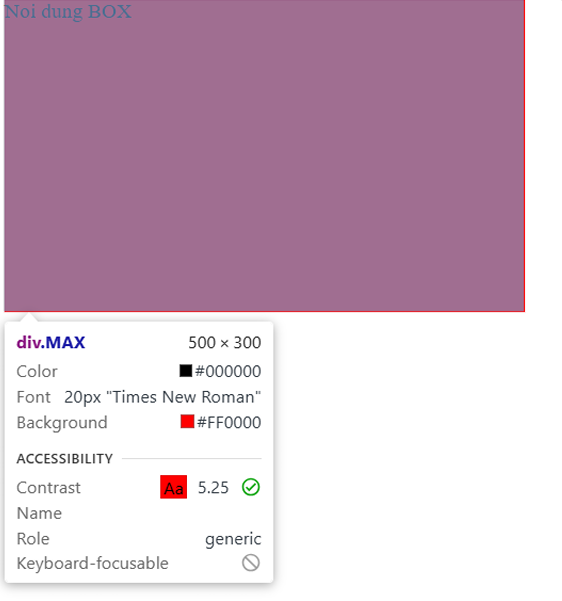
\includegraphics[height=6.2cm, keepaspectratio]{figures/max_width_devtools_wide_500px_clean.png}}
    \caption{Viewport rộng ($> 500\text{px}$): Khóa tại $500\text{px} \times 300\text{px}$}
    \label{subfig:devtools_wide}
\end{subfigure}
\caption{Hình Ảnh Chụp Thực Tế Chrome DevTools: Đối Chiếu Kích Thước Đo Lường Của Lớp .MAX}
\label{fig:max_width_devtools_comparison}
\end{figure}

\subsubsection{Cải Tiến Hoàn Hảo Cho Responsive}
Nếu bạn muốn phần tử khối co giãn mượt mà hơn và luôn bám dính $100\%$ không gian khi màn hình nhỏ, hãy kết hợp thêm thuộc tính \codeinline{width: 100\%;}:

\begin{codeWindow}[Mẫu Thiết Kế .MAX Hoàn Thiện Tối Ưu Cho Responsive]
\begin{lstlisting}[language=CSS3]
.MAX {
    background: red;
    width: 100%;        /* Chiay 100% khi man hinh nho hon 500px */
    max-width: 500px;   /* Chan lai khong cho lon hon 500px tren man hinh lon */
    height: 300px;
    font-size: 20px;
}
\end{lstlisting}
\end{codeWindow}

% ------------------------------------------------------------------------------
% 4.6 KHI NÀO DÙNG MAX-WIDTH & TỔNG KẾT
% ------------------------------------------------------------------------------
\subsection{6. Khi Nào Dùng max-width? \& Bảng Tổng Hợp Giá Trị Thường Dùng}
\label{subsec:when_to_use_max_width}

\begin{prettyTableBox}[Bảng Tra Cứu Các Giá Trị Thường Dùng Của Thuộc Tính max-width]
\rowcolors{2}{white}{primaryBlue!4}
\sffamily\small
\begin{tabularx}{\linewidth}{|>{\raggedright\arraybackslash \ttfamily\color{primaryBlue}\bfseries}K{2.8cm}|Z|}
\hline
\rowcolor{primaryBlue} \thd{\sffamily Giá trị} & \thd{\sffamily Ý nghĩa \& Ngữ cảnh sử dụng} \\
\hline
px & Giới hạn chiều rộng tối đa theo đơn vị pixel tuyệt đối (ví dụ: \codeinline{max-width: 800px;}). Rất phổ biến cho card, form đăng nhập, container. \\
\hline
\% & Giới hạn theo tỷ lệ phần trăm so với phần tử cha (ví dụ: \codeinline{max-width: 100\%;}). Tiêu chuẩn vàng để chống tràn cho ảnh và video. \\
\hline
em, rem & Giới hạn kích thước theo độ lớn phông chữ. Cực kỳ tối ưu cho các cột đọc báo để giữ độ dài dòng từ 65 đến 75 ký tự. \\
\hline
vw & Giới hạn theo tỷ lệ phần trăm chiều rộng của màn hình (\term{viewport}). \\
\hline
none & Giá trị mặc định của CSS. Phần tử không có bất kỳ giới hạn chiều rộng tối đa nào. \\
\hline
\end{tabularx}
\end{prettyTableBox}

\subsubsection{Khi Nào Bắt Buộc Phải Dùng max-width?}
\begin{enumerate}[leftmargin=1.5em, itemsep=3pt, parsep=0pt]
    \item \textbf{Khi muốn giới hạn phần tử không quá lớn nhưng vẫn tự co lại nếu cần}: Tránh làm mất cân đối thị giác trên các màn hình máy tính để bàn có độ phân giải cao.
    \item \textbf{Khi thiết kế giao diện responsive trên nhiều kích thước màn hình}: Đảm bảo trải nghiệm đồng nhất trên cả Desktop, Tablet và Mobile.
    \item \textbf{Khi muốn nội dung tự động thu nhỏ trên màn hình nhỏ mà không bị vỡ}: Loại bỏ vĩnh viễn nguy cơ sinh thanh cuộn ngang gây ức chế cho người dùng.
\end{enumerate}

\begin{tipBox}[Lưu Ý Vàng Khi Sử Dụng Thuộc Tính max-width]
\begin{itemize}[leftmargin=1.5em, itemsep=2.5pt, parsep=0pt]
    \item \textbf{Luôn kết hợp với \codeinline{width: 100\%;}}: Để phần tử tự do co giãn linh hoạt khi không gian nhỏ hơn giá trị \codeinline{max-width}.
    \item \textbf{Không làm phần tử nhỏ hơn}: Giá trị \codeinline{max-width} chỉ giới hạn kích thước trần lớn nhất, không ép phần tử phải co lại nếu nội dung tự nhiên của nó vốn đã nhỏ.
    \item \textbf{Kết hợp với \codeinline{margin: 0 auto;}}: Để đưa khối giao diện vào chính giữa màn hình một cách cân đối và chuyên nghiệp.
    \item \textbf{Đối tượng áp dụng thường xuyên}: Khung chứa nội dung (\codeinline{.container}), hình ảnh (\codeinline{<img>}), biểu mẫu nhập liệu (\codeinline{<form>}), thẻ bài viết (\codeinline{.card}), và hộp thoại pop-up (\codeinline{.modal}).
\end{itemize}
\end{tipBox}

% ==============================================================================
% MỤC 5: CHUYÊN ĐỀ THỰC CHIẾN: LÀM CHỦ THUỘC TÍNH MAX-HEIGHT
% ==============================================================================
\clearpage
\section{Chuyên Đề Thực Chiến: Làm Chủ Thuộc Tính \csshint{max-height}}
\label{sec:max_height_masterclass}

Trong thiết kế giao diện web hiện đại, việc kiểm soát chiều cao của phần tử luôn tiềm ẩn nhiều thách thức hơn so với chiều rộng. Nội dung văn bản có thể dài ngắn bất định tùy thuộc vào dữ liệu động hoặc ngôn ngữ người dùng. Thuộc tính \codeinline{max-height} chính là công cụ đắc lực giúp lập trình viên vừa giới hạn được kích thước trần an toàn, vừa bảo toàn tính co giãn linh hoạt tự nhiên theo nội dung.

% ------------------------------------------------------------------------------
% 5.1 KHÁI NIỆM & CƠ CHẾ HOẠT ĐỘNG
% ------------------------------------------------------------------------------
\subsection{Bản Chất \& Cơ Chế Hoạt Động Của \csshint{max-height}}
\label{subsec:max_height_concept}

\begin{conceptBox}[Định Nghĩa Chuẩn: Thuộc Tính max-height]
Thuộc tính \codeinline{max-height} trong CSS dùng để \textbf{giới hạn chiều cao tối đa} mà một phần tử có thể đạt được:
\begin{itemize}[leftmargin=1.2em, itemsep=3pt, parsep=0pt]
    \item \textbf{Nếu nội dung ít hơn giới hạn}: Phần tử sẽ tự động co lại đúng bằng chiều cao tự nhiên của nội dung (với điều kiện \codeinline{height: auto;}).
    \item \textbf{Nếu nội dung vượt quá giới hạn}: Chiều cao phần tử bị chặn cứng tại giá trị \codeinline{max-height}. Phần nội dung tràn ra ngoài sẽ được xử lý tùy theo thuộc tính \codeinline{overflow} đi kèm (cắt bỏ, tràn đè hoặc sinh thanh cuộn).
\end{itemize}
\end{conceptBox}

\subsubsection{Cú Pháp Khai Báo \& Đơn Vị}

\begin{codeWindow}[Cú Pháp Cơ Bản Thuộc Tính max-height]
\begin{lstlisting}[language=CSS3]
selector {
    max-height: value;
}
\end{lstlisting}
\end{codeWindow}

Trong đó, \codeinline{value} có thể nhận các giá trị:
\begin{itemize}[leftmargin=1.5em, itemsep=3pt, parsep=0pt]
    \item \textbf{Đơn vị đo lường}: \codeinline{px}, \codeinline{em}, \codeinline{rem}, \codeinline{vh}, \codeinline{vw}, \codeinline{\%}.
    \item \textbf{Từ khóa đặc biệt}: \codeinline{none} (mặc định -- không giới hạn chiều cao tối đa).
\end{itemize}

\begin{codeWindow}[Ví Dụ Cơ Bản Thiết Lập max-height]
\begin{lstlisting}[language=CSS3]
.box {
    background: #e74c3c;
    max-height: 300px;
    width: 500px;
}
\end{lstlisting}
\end{codeWindow}

\begin{itemize}[leftmargin=1.5em, itemsep=3pt, parsep=0pt]
    \item Nếu khối \codeinline{.box} chứa lượng nội dung ngắn có chiều cao dưới $300\text{px}$, nó sẽ tự co lại ôm sát nội dung.
    \item Nếu khối chứa lượng nội dung đồ sộ vượt quá $300\text{px}$, phần tử sẽ dừng lại ở đúng ngưỡng $300\text{px}$.
\end{itemize}

\begin{figure}[H]
\centering
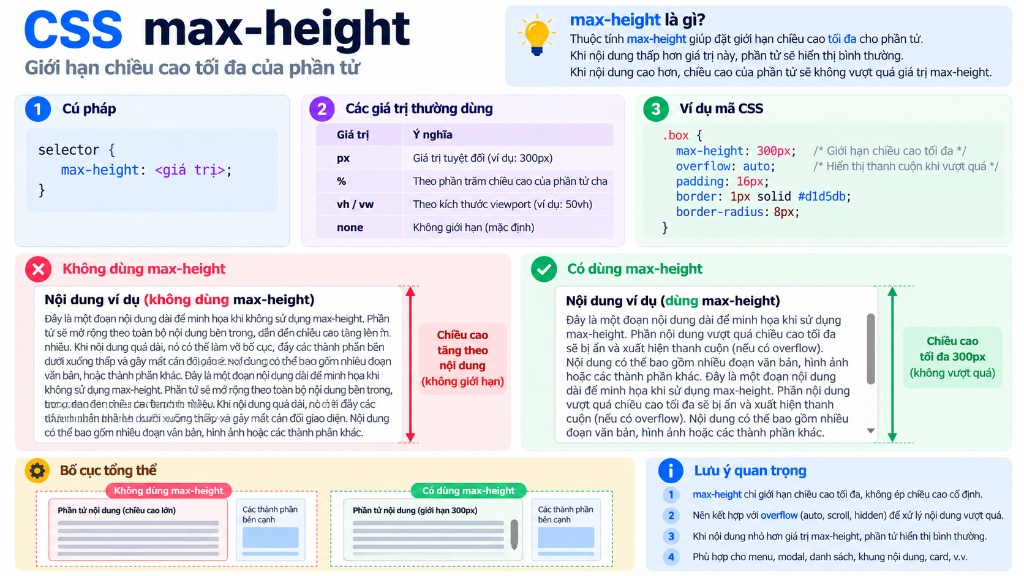
\includegraphics[width=\linewidth]{figures/css_max_height_overview_infographic.jpg}
\caption{Infographic Tổng Quan Thuộc Tính CSS \codeinline{max-height}: Cú Pháp, Bảng Giá Trị, Mã Mẫu \& Đối Chiếu Bố Cục}
\label{fig:css_max_height_overview_infographic}
\end{figure}

% ------------------------------------------------------------------------------
% 5.2 SO SÁNH HEIGHT VS MAX-HEIGHT
% ------------------------------------------------------------------------------
\subsection{So Sánh Toàn Diện Giữa \csshint{height} Và \csshint{max-height}}
\label{subsec:height_vs_max_height}

Sự khác biệt căn bản giữa hai thuộc tính này nằm ở \textbf{tính linh hoạt đối với dung lượng nội dung}:

\begin{prettyTableBox}[Bảng So Sánh Chi Tiết: height vs max-height]
\rowcolors{2}{white}{primaryBlue!4}
\sffamily\small
\begin{tabularx}{\linewidth}{|>{\raggedright\arraybackslash \ttfamily\color{primaryBlue}\bfseries}K{2.8cm}|Z|Z|}
\hline
\rowcolor{primaryBlue} \thd{\sffamily Tiêu chí} & \thd{\sffamily height} & \thd{\sffamily max-height} \\
\hline
Cơ chế cốt lõi & Khóa cứng chiều cao của phần tử tại một kích thước cố định. & Thiết lập ngưỡng trần tối đa; phần tử vẫn tự do co giãn nhỏ hơn. \\
\hline
Khi nội dung ít & Phần tử \textbf{vẫn giữ nguyên} kích thước cố định, tạo ra khoảng trống thừa thãi lãng phí. & Phần tử \textbf{tự co lại} vừa vặn theo nội dung, tiết kiệm không gian giao diện. \\
\hline
Khi nội dung nhiều & Phần tử bị tràn (\term{overflow}) ra ngoài hoặc bị che khuất nội dung. & Phần tử đạt ngưỡng chặn trần, dễ dàng kết hợp \codeinline{overflow: auto;} để cuộn. \\
\hline
Mức độ linh hoạt & Kém linh hoạt, dễ gây vỡ bố cục trên màn hình nhỏ. & Cực kỳ linh hoạt, chuẩn mực vàng cho thiết kế đáp ứng (\term{Responsive}). \\
\hline
\end{tabularx}
\end{prettyTableBox}

\begin{codeWindow}[Mã Nguồn So Sánh .box1 (height) vs .box2 (max-height)]
\begin{lstlisting}[language=CSS3]
/* Hop 1: Luon luon cao dung 300px bat ke noi dung chi co 1 dong chu */
.box1 {
    height: 300px;
    background: #3498db;
}

/* Hop 2: Co gian linh hoat theo chu, toi da chi dat 300px */
.box2 {
    max-height: 300px;
    height: auto;
    background: #2ecc71;
}
\end{lstlisting}
\end{codeWindow}

% ------------------------------------------------------------------------------
% 5.3 MINH HỌA THỰC NGHIỆM: MAX-HEIGHT CO GIÃN THEO NỘI DUNG
% ------------------------------------------------------------------------------
\subsection{Thực Nghiệm Thực Tế: \csshint{max-height} Phụ Thuộc Vào Nội Dung}
\label{subsec:max_height_content_dependency}

Khi sử dụng \codeinline{max-height}, phần tử sẽ co giãn nhịp nhàng theo lượng chữ bên trong. Hãy cùng đối chiếu hai trường hợp thực tế dưới đây:

\begin{figure}[H]
\centering
\begin{subfigure}[b]{\linewidth}
    \centering
    \setlength{\fboxsep}{1pt}\setlength{\fboxrule}{0.8pt}
    \fcolorbox{gray!30}{white}{
\includegraphics[width=0.95\linewidth]{figures/max_height_content_short.png}}
    \caption{Trường hợp 1: Nội dung ít (1 dòng chữ) $\rightarrow$ Khối tự co lại siêu mỏng ôm sát dòng chữ.}
    \label{subfig:max_height_short}
\end{subfigure}\\[0.4cm]
\begin{subfigure}[b]{\linewidth}
    \centering
    \setlength{\fboxsep}{1pt}\setlength{\fboxrule}{0.8pt}
    \fcolorbox{gray!30}{white}{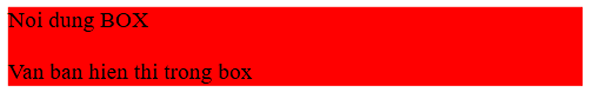
\includegraphics[width=0.95\linewidth]{figures/max_height_content_long.png}}
    \caption{Trường hợp 2: Bổ sung thêm dòng nội dung $\rightarrow$ Khối tự động nới rộng chiều cao theo nội dung.}
    \label{subfig:max_height_long}
\end{subfigure}
\caption{Thực Nghiệm Trực Quan: Chiều Cao Thực Tế Của Khối Co Giãn Theo Nội Dung Dù Đang Đặt \codeinline{max-height: 300px;}}
\label{fig:max_height_real_experiment}
\end{figure}

% ------------------------------------------------------------------------------
% 5.4 CẠM BẪY THỰC CHIẾN: XUNG ĐỘT GIỮA HEIGHT VÀ MAX-HEIGHT
% ------------------------------------------------------------------------------
\subsection{Cạm Bẫy Thực Chiến: Xung Đột Giữa \csshint{height} Cố Định Và \csshint{max-height}}
\label{subsec:conflict_height_max_height}

Một lỗi rất phổ biến mà nhiều lập trình viên mới gặp phải là khai báo đồng thời cả \codeinline{height} và \codeinline{max-height} cùng một con số:

\begin{warnBox}[Cạm Bẫy: Vô Hiệu Hóa max-height Khi Dùng Chung Với height Cố Định]
\begin{lstlisting}[language=CSS3]
.MAX {
    background: red;
    width: 500px;
    height: 300px;      /* Khoa cung chieu cao 300px */
    max-height: 300px;  /* Gioi han tran 300px -> HOAN TOAN VO TAC DUNG! */
    font-size: 20px;
}
\end{lstlisting}
\textbf{Nguyên nhân}: Khi bạn đã ấn định \codeinline{height: 300px;}, phần tử đã bị khóa cứng ở $300\text{px}$. Do đó, việc đặt thêm \codeinline{max-height: 300px;} là hoàn toàn dư thừa vì phần tử không còn khả năng co giãn nữa!
\end{warnBox}

\subsubsection{Giải Pháp Chuẩn Kỹ Thuật: Sử Dụng \csshint{height: auto;}}

Để \codeinline{max-height} phát huy toàn bộ sức mạnh, bạn phải cho phép phần tử được tự do co giãn bằng cách thiết lập \codeinline{height: auto;} (hoặc không khai báo thuộc tính \codeinline{height}):

\begin{codeWindow}[Giải Pháp Khắc Phục Chuẩn Kỹ Thuật]
\begin{lstlisting}[language=CSS3]
.MAX {
    background: red;
    width: 500px;
    max-height: 300px;  /* Tran chieu cao toi da 300px */
    height: auto;       /* Co gian tu do theo noi dung */
    font-size: 20px;
    overflow: auto;     /* Tu dong cuon neu vuot qua 300px */
}
\end{lstlisting}
\end{codeWindow}

\begin{itemize}[leftmargin=1.5em, itemsep=3pt, parsep=0pt]
    \item \textbf{Nếu nội dung ít}: Khối \codeinline{.MAX} sẽ nhỏ hơn $300\text{px}$, ôm sát chữ.
    \item \textbf{Nếu nội dung nhiều}: Khối \codeinline{.MAX} dừng lại ở $300\text{px}$ và sinh thanh cuộn dọc mượt mà.
\end{itemize}

% ------------------------------------------------------------------------------
% 5.5 CÁC ỨNG DỤNG THỰC TẾ CỦA MAX-HEIGHT
% ------------------------------------------------------------------------------
\subsection{Các Ứng Dụng Thực Tế Tiêu Biểu Của \csshint{max-height}}
\label{subsec:practical_apps_max_height}

\subsubsection{Ứng Dụng 1: Kết Hợp Với \csshint{overflow} Tạo Khung Cuộn Danh Sách Thông Báo}

Khi xây dựng giao diện bảng điều khiển (\term{Dashboard}), danh sách thông báo hoặc khung bình luận thường có độ dài biến động. Nếu không giới hạn chiều cao, danh sách dài sẽ đẩy toàn bộ nội dung khác xuống dưới làm vỡ bố cục trang:

\begin{figure}[H]
\centering
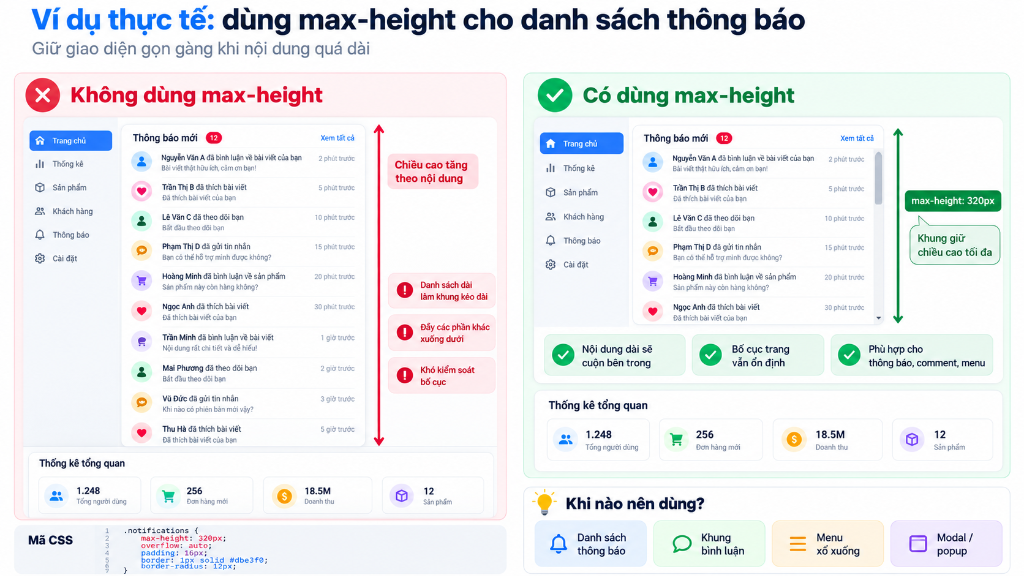
\includegraphics[width=\linewidth]{figures/max_height_notification_dashboard.png}
\caption{Ví Dụ Thực Tế: Ứng Dụng \codeinline{max-height: 320px;} Giữ Khung Thông Báo Luôn Gọn Gàng \& Ổn Định Bố Cục Trang}
\label{fig:max_height_notification_dashboard}
\end{figure}

\begin{codeWindow}[Mã Nguồn Khung Thông Báo Chuẩn Dashboard Với max-height]
\begin{lstlisting}[language=CSS3]
.notifications {
    max-height: 320px;
    overflow: auto;
    padding: 16px;
    border: 1px solid #dbe3f0;
    border-radius: 12px;
}
\end{lstlisting}
\end{codeWindow}

\subsubsection{Ứng Dụng 2: Tạo Hiệu Ứng Mở Rộng / Thu Gọn Mượt Mà (Accordion Transition)}

Trong CSS, bạn \textbf{không thể} áp dụng hiệu ứng chuyển động (\codeinline{transition}) trực tiếp từ \codeinline{height: 0;} lên \codeinline{height: auto;}. Cách giải quyết kinh điển là kết hợp \codeinline{max-height} và \codeinline{transition}:

\begin{codeWindow}[Tạo Hiệu Ứng Accordion Mượt Mà Không Cần JavaScript]
\begin{lstlisting}[language=CSS3]
.accordion-content {
    max-height: 0;                          /* Ban dau thu gon hoan toan */
    overflow: hidden;                       /* An phan noi dung bi thu gon */
    transition: max-height 0.4s ease-in-out;/* Hieu ung chuyen dong muot ma */
}

/* Khi hover hoac khi co class kich hoat */
.accordion-item:hover .accordion-content {
    max-height: 400px;                      /* Mo rong den nguong du chua noi dung */
}
\end{lstlisting}
\end{codeWindow}

% ------------------------------------------------------------------------------
% 5.6 KHI NÀO NÊN DÙNG & LƯU Ý VÀNG
% ------------------------------------------------------------------------------
\subsection{Khi Nào Nên Dùng \csshint{max-height} \& Lưu Ý Thực Chiến}
\label{subsec:when_to_use_max_height}

\begin{tipBox}[4 Trường Hợp Vàng Nên Sử Dụng max-height]
\begin{enumerate}[leftmargin=1.5em, itemsep=3pt, parsep=0pt]
    \item \textbf{Giới hạn chiều cao an toàn}: Không làm mất đi tính co giãn linh hoạt tự nhiên của phần tử.
    \item \textbf{Hiển thị thanh cuộn tự động}: Xử lý các khối nội dung người dùng sinh ra (\term{User Generated Content}) có độ dài khó lường.
    \item \textbf{Hiệu ứng chuyển động}: Làm Accordion, Dropdown Menu, Collapsible Panels bằng CSS thuần.
    \item \textbf{Tối ưu hóa Responsive}: Giữ các khối hình ảnh/video không vượt quá độ cao màn hình điện thoại (ví dụ: \codeinline{max-height: 80vh;}).
\end{enumerate}
\end{tipBox}

\begin{warnBox}[3 Lưu Ý Sống Còn Khi Dùng max-height]
\begin{itemize}[leftmargin=1.5em, itemsep=3pt, parsep=0pt]
    \item \textbf{Không đặt \codeinline{max-height: none;}} nếu đang muốn hạn chế chiều cao, vì \codeinline{none} là giá trị hủy bỏ giới hạn.
    \item \textbf{Cẩn thận với \codeinline{overflow: hidden;}}: Nếu nội dung dài hơn \codeinline{max-height}, toàn bộ phần tràn sẽ bị cắt cụt vĩnh viễn và người dùng không thể đọc được nếu không có cơ chế mở rộng.
    \item \textbf{Khi làm hiệu ứng transition}: Tránh chuyển từ \codeinline{max-height: 0} sang \codeinline{none}; thay vào đó hãy đặt một giá trị cụ thể ước lượng vừa đủ lớn (ví dụ: \codeinline{500px} hoặc \codeinline{1000px}).
\end{itemize}
\end{warnBox}

\end{document}
